\documentclass{report}
%使用ctex宏包将标题设置为中文格式,ctex和documentclass 其中一个,否则冲突
\usepackage[UTF8, heading = true,scheme=chinese]{ctex}
\ctexset{
	section={
		name={第,节},
		number=\arabic{section}, },
		section/titleformat+={\zihao{4}\raggedright}
}


\usepackage{graphicx}
\graphicspath{ {/Users/sun/Desktop/NBA/MyLatex/figure/}}
\usepackage[a4paper,top=20mm,bottom=20mm]{geometry}
\usepackage{fancyhdr}
\pagestyle{fancy}
\fancyhf{}
\fancyhead[LE,RO]{西南大学数学与统计学院}
\fancyhead[RE,LO]{NBA球员数据对球队胜率影响}
\usepackage{amsmath}
\usepackage{subcaption}
\usepackage{listings}
%插入参考文献
\usepackage{apacite}
\renewcommand\refname{参考文献}
\usepackage{url}

\usepackage{abstract}
\renewcommand{\abstractname}{\LARGE 摘要}
\begin{document}
	
	\begin{titlepage}
		\centering
		
\includegraphics[width=0.5\textwidth]{university.jpg}\par
		\vspace{1cm}
		{\scshape\LARGE 本科毕业论文 \par}
		\vspace{1cm}
		{\scshape\LARGE\bfseries 题目:NBA球员数据对球队胜率的影响\par}
		\vspace{1cm}
		{\large 学院:数学与统计学院\par}
		\vspace{0.5cm}
		{\large 专业: 统计学\par}
		\vspace{0.5cm}
		{\large 年级: 2016级\par}
		\vspace{0.5cm}
		{\large 学号:222016314032025\par}
		\vspace{0.5cm}
		{\large 姓名: 孙瑶\par}
		\vspace{0.5cm}
		{\large 指导老师: 李婷婷\par}
		\vspace{0.5cm}
		{\large 成绩:\par}
		
		\vfill
		
		% Bottom of the page
		{\large \today\par}
	\end{titlepage}
	
	\begin{abstract}
		本文利用NBA球员在18-19赛季中基本数据,构建衡量球员效率、有效利用率、实际命中率、控球时长等指标,然后根据每位球员在整个赛季中的上场时间作为权重,将球员指标加权平均后构建某队球员对所在球队的实际贡献指标,综合球队的进攻效率,防守效率和净得分等指标,找到对球队在比赛中获胜概率的主要影响因素,为球队在制定训练计划,安排球员配置等方面提出有效建议,并建立对球队在下一赛季胜率的预测模型。本文首先对NBA篮球赛制和特点进行总结,分析出影响球队胜率的最主要因素,提取变量特征,建立多元线性回归模型,以下一赛季的数据作为测试集计算出每个球队在下一个赛季中的胜率,并返回最终预测结果\\
		
		\textbf{关键词: 多元回归模型、指标构建、相关性分析、PER、TSR、eFGR}\\
		
		Based on NBA players basic data in the 18th and 19th season, construct measure player efficiency, effective utilization and the actual shooting, ball control indices such as the length, then according to each player of the season playing time as the weight, the weighted average players indexes after building a team player on the team's actual contribution index, comprehensive efficiency of the team's offensive, defensive efficiency and net classification index, find the probability of winning in the game to the team's main influence factors, in the training plan for the team, suggest effective arrangements for the player configuration, and establish the forecast model of team next season match. This paper first summarizes the NBA basketball game system and characteristics, analyzes the most important factors affecting the team's winning rate, extracts the characteristics of variables, and establishes a multiple linear regression model. The following season's data is used as a test set to calculate the winning rate of each team in the next season, and returns the final prediction results.\\
		
		\textbf{Keywords: Multi-linear Regression Model、 Metrics Construction、Correlation analysis、PER、 TSR、eFGR}
	\end{abstract}
	
	
		

	\tableofcontents
	\newpage
	\section{研究目的}
	不久之前,金州勇士队通过分析大量的NBA赛事数据和观看大量的球队比赛,找到了防守安东尼·戴维斯的最佳球员。在最新的一赛季比赛中,勇士队的表现有了新的飞跃和突破。今年,几乎NBA每一支球队都开始追踪其球员的比赛数据,包括运动员在场上的得分位置,或者每个队员的比赛数据等。通过有效的数据分析,高级的数据模型,和分析工具,NBA比赛已经逐渐转化为专业篮球比赛。这样的转变不仅影响着球员的打球习惯,教练的训练方法,粉丝与球星的互动方式,甚至在赛制上也有了不同的调整运动员,教练,粉丝,甚至NBA分析员都希望好好利用大量的数据,来满足他们不同的需求。



篮球比赛在每个常规赛季中进行82场比赛。网上公开了大量的比赛数据,也有很多写得很好的文章和书籍分析球队球员表现.但是专业分析员会利用每场比赛球员的走位,和一些不对外公开的数据进行更具体详细的分析。由于数据的有限性,本位会利用网上公开的球员和球队数据进行分析,探索个体球员表现和球队表现的关系,本文最终目的是根据每队球员的具体数据预测NBA球队在季后赛的表现。


近几年,衡量球员表现的指标数据在近几年间不断更新,更加全面的反映球员的表现。最基本且最容易获得的数据是每个球员和球队每场比赛的得分数据。得分数据不仅记录某个球员和他队友的各项得分,还记录了他的对手球队和球员的防守数据。之前,得分数据仅仅包含最基础的球员数据,包括球员进球得分,篮板球,助攻数,和投篮命中率等。但这些数据来衡量一个球员的表现,能力和价值是远远不够的。首先,现有的统计量更多偏向记录球员的进攻数据,而忽视了球员的防守贡献水平;如果这个球员在整场比赛中投篮次数更多,助攻更多,这个球员可能是更有价值的球员,但尽管他有很强的的防守能力,比如他多次抢断对方投球,或盖帽,他也不一定能有很高的综合评分。其次,现有的统计数据可能对在场上拥有更多控球权的球员更有利;比如控球后卫将球带到前场并且更多的组织进攻,他带球时间更长,所以他的综合数据可能就更优秀。但是一个球员的控球能力却没有很精准的数据衡量,但控球能力是一个很重要的衡量指标。因此联盟从1970-1971年的赛季之后,开始记录球员的犯规数。


至今,由于有了更精准的记录仪器,我们可以获得更准确地球员数据,进行更具体的数据分析。例如金州勇士队,就大量利用大数据分析对球队整体训练计划和决策等方面进行改正。本文不会用到每一个球员在场上的实时位置信息和训练信息等十分具体的数据进行预测,因为这些数据不是对大众公开的。但是本文将会运用更常见的统计指标如射门得分,助攻次数,抢断次数,盖帽次数等,通过分析这些指标对球员和球队贡献的重要性来预测该球队的输赢。
	
	\section{研究背景}
	

在高级篮球分析领域,研究人员记录和跟踪运动员的身体数据可以制定出更合适的训练方法,对十分有价值的球员可以针对他设计出一个更能够辅助他得到更多分数的球队阵容从而为球队赢得更多的比赛;在娱乐领域,观众可以根据NBA官网公布的球员球队数据和信息,计算和预测球队的胜负。本文希望根据个体球员在比赛中的的基本数据得到反映其对所在球队贡献程度的指标,即衡量球员价值的指标,综合某个球队所有球员的贡献,得到球队的整体实力,从而根据球队的整体数据对下一个赛季中球队的胜率进行预测。
	
	\section{数据说明}
	本文采用的是近2018-19年常规赛季的公开数据进行建模。由于比赛从赛制,到规则等各个方面都随着时代不断改变,甚至评判输赢的规则都有改变;尽管目前可以收集到自从1946-47赛季开始至今的所有赛事数据,之前的数据对现在比赛的分析也没有太多可借鉴作用。所以我们用今年来的所有常规赛事所公开的数据进行分析与建模。比如在上世纪末期,一个球队的输赢很大程度取决于个头最大的球员(如中风和大前锋),因为当时比赛的节奏相对较慢,主导比赛进程的球员通常是个头大的球员;但是如今,比赛节奏越来越快,比赛进程也更趋于数据化,专业化和技术化,这就为身形较小而灵活,但是技术水平很高,如投篮水平很高,控球能力很强的球员如史蒂芬库里,詹姆斯哈登,凯利欧文等身高不出众但命中率很高的球员。但联盟赛制转变后更有利于进攻型球员,尤其是擅长投射的球员,这使得比赛更激动人心,吸引更多观众的目光。\cite{fixler2012fading}
\begin{table}[h!]
	\begin{center}
		\begin{tabular}{ |c|c|c| } 
			\hline
			变量名 &	变量含义(英文)&	变量含义(中文)
\\
			\hline
			Rk	&Rank&	排名
\\
			Pos	&Position&	首发位置
\\
			Age	&Player's age&	年龄
\\
			Tm	&Team&	所在球队
\\
			G&	Games	&该赛季比赛总场数
\\
			MP&	Minutes Played&	球员上场时长
\\
			FG&	Field Goals	&球员投篮命中
\\
			FGA	&Field Goals Attempts&	球员投篮
\\
			FG\%	&Field Goal Percentage&	场均球员命中率
\\
			3P&	3-Point Field Goals	&场均3分球命中得分次数
\\
			3PA	&3-Point Field Goal Attempts&	场均3分球投篮次数
\\
			3P\%&	FG\% on 3-Pt FGAs&	场均3分球得分率
\\
			2P&	2-Point Field Goals	&场均2分球命中得分次数
\\
			2PA&	2-point Field Goal Attempts&	场均2分球投篮次数
\\
			2P\%&	FG\% on 2-Pt FGAs.&	场均2分球得分率
\\
			eFG\%&	Effective Field Goal Percent&	场均有效的投篮得分率
\\
			FT&	Free Throws	&场均罚球得分
\\
			FTA	&Free Throw Attempts&	场均罚球投篮次数
\\
			FT\%	&Free Throw Percentage&	场均罚球命中率
\\
			ORB	&Offensive Rebound	&场均进攻篮板球次数
\\
			DRB&	Defensive Rebounds	&场均防守篮板球次数
\\
			TRB	&Total Rebounds	&场均篮板球总次数
\\
			AST&	Assists	&场均助攻次数
\\
			STL	&Steals	&场均盖帽次数
\\
			BLK	&Blocks	&场均抢断次数
\\
			TOV	&Turnovers	&场均失误次数
\\
			PF&	Personal Fouls	&场均个人犯规次数
\\
			PTS&	Points	&场均得分
\\
			\hline
		\end{tabular}
		\caption{每个赛季所有球员的整体数据}
		\label{tab:1}
	\end{center}
\end{table}


\begin{table}[t]
	\centering
	\begin{tabular}{|c|c|c|}
		\hline
		变量名	&英文名称&	中文解释
\\
		\hline
		Rk&	Rank&	球队在赛季中的排名
\\
		W&	Wins&	球队整赛季赢过的比赛
\\
		W/L\%&	Win-Loss Percentage&	球队的胜负率
\\
		MOV	&Margin of Victory&	输赢球队比分之差
\\
		Ortg	&Offensive Rating&	每100次进攻的得分
\\
		DRtg&	Defensive Rating&	每100次进攻的失分
\\
		NRtg&	Net Rating&	每100次进攻机会的净胜分
\\
		MOV/A&	Adjusted Margin of Victory&	根据对手进攻节奏调整后的MOV
\\
		Ortg/A	&Adjusted Offensive Rating&	根据对手进攻节奏调整后的每100次进攻得分
\\
		DRtg/A&	Adjusted Defensive Rating	&根据对手进攻节奏调整后的失分
\\
		NRtg/A&	Adjusted Net Rating	&根据对手进攻节奏调整后的净胜分
\\
		\hline
	\end{tabular}
	\caption {每个赛季所有球员的整体数据}
	\label{2}
	
\end{table}


\begin{enumerate}
	\item  以2018-19赛季比赛中球员数据为例,如表\ref{tab:1}
	\item 2018-19赛季比赛中球队数据为例,如表\ref{2}
	\item 收集每个球队的整个赛季中与之对抗的球队的比赛数据,变量名如\ref{tab:1}。
	\item 收集每个球队在整个赛季中数据统计,变量名如\ref{tab:1}.

\end{enumerate}






	
	\section{指标设计}
	上述篮球的基础数据是观众了解一个球员,球队的最直观方法也是观看比赛后评估一个球员表现的最直观的方法,但是Mark Cuban认为在专业篮球运动员分析某球队和某球员的具体表现和如何提高球队比赛效率,提高球员有效得分率,提高球员价值上仅仅利用简单的基础数据是远远不够的。这时需要利用数据来建立高级篮球分析指标,而这些指标可能对观众来说是没有实际意义的。本文将提取教练或篮球分析员最关注的指标:本文的指标构建分为两部分:第一部分是个体球员的指标构建,主要是在基础篮球数据的 基础上根据需求设计高级指标,在衡量运动员水平的时候包括衡量球员价值、球员效率、球员控球、球员实际命中率、球员有效得分率等;然后将个体球员数据整合到其球队的数据中,代表该球队整体球员的指标;第二部分考虑球队指标,球队指标包括球队排名、球队比分差距、球队的攻守效率,和作为我们预测结果的球队胜率:




\begin{enumerate}
	\item 个体球员指标:
	\begin{enumerate}
	
		
		
		
		
	
	
		\item True Shooting Percentage实际命中率:实际命中率等于个体球员在场上的总得分,除以运动员在赛场上所有投篮次数和罚球次数应得的分数 \\
		相对于衡量一个球员所有的投篮命中率,实际命中率更全面涵盖一个球员通过投篮得到所有的分数,包括二分球,三分球和罚球得分,该指标可以很客观的评判运动员的命中率高低,从而衡量一个球员的命中率对球队的贡献。\\
		
		\begin{align}
			True shooting Rate =  \frac{Points}{2*(Field Goal Attempt + 0.44*Free Throw Attempt)}
		\end{align}
		注释:系数0.44是根据一个球员每100次控球中2分球和3分球的出手比例计算而来的。如果100次控球中所有的投篮都是2分球,该系数应该是0.5,如果100次控球中所有投篮出手都是3分球,该系数为0.333.
	
		\item Effective Field Goal Percentage有效得分率:得分效率是每个球员在场上除了罚球命中之外的投球命中除以总投球次数,这里假设除了投球以外的命中得分均分为2分,所以利用总得分减去罚球得分除以2来近似所有除去罚球之后的投球命中次数。\\由于衡量命中率之后需要考虑每次命中的实际得分,由于3分球出手命中后得3分,2分球出手后命中得2分,不能用统一的标准来计算所有命中的得分。计算有效得分率,可以更好的衡量球员得分对整体球队的贡献。
		
		\begin{align}
		eFG Rate = \frac{(Points-FT)/2}{FGA}
		\end{align}
	
		\item PER:\cite{hollinger2005pro}衡量球员效率的指标Per Efficiency Rating. 指标根据NBA官网公开的各球员、球队、联盟的基础数据计算得出。总结球员对球队的正向贡献和负向贡献,即在衡量球员得分的指标前赋予一个正的系数,在衡量球员失分的指标前赋予一个负的系数,再将所有加权后的指标相加,再除以根据球队和联盟数据构建的指标对球员的数据进行规范化。PER最终得到球员每分钟的贡献率,该指标不应该受到球员上场时间,球队进攻类型,整个联盟赛制变化的影响。该指标客观有效的衡量球员的比赛效率,可以成为衡量球员对球队贡献指标之一。\\ 首先定义三个参数:
		\begin{align}
			Factor &= \frac{2}{3} - \frac{(0.5 * (League Assists / League Field Goal))}{(2 * (League Field Goal / League Free Throw))}\\
			DRB\%   &=  \frac{(League Total Rebounds - League Offensive Rebound)}{League Total Rebounds}
		\end{align}
		
		\begin{multline}
			VOP   =  League Points / (League Field Goal Attempt - League Offensive Rebound \\+ League Turnovers + 0.44 * League FreeThrowAttempts)
		\end{multline}
 依据上述三个参数,我们定义PER指标的计算公式
 \begin{multline}
 uPER = (1 / Minue Play) *
 [ 3Point
 + (2/3) * Assists
 \\+ (2 - Factor  * (Team Assists / Team Field Goal)) * Field Goal
 \\+ (Free Throw *0.5 * (1 + (1 - (Team Assists / Team Field Goal)) \\+ (2/3) * (Team Assists / Team Field Goal)))
 \\- VOP * Turnovers
 - VOP * DRB\%* (Field Goal Attempt - Field Goal)
 \\- VOP * 0.44 * (0.44 + (0.56 * DRB)) * (Free Throw Attempt - Free Throw)
 \\+ VOP * (1 - DRB\%) * (TotalRebound - Offensive Rebound)
 \\+ VOP * DRB\% * Offensive Rebound
 + VOP * Steal
 + VOP * DRB\% * Block
 \\- Personal Fouls * ((League Free throw / League Personal Fouls) - \\0.44 * (League FreeThrowAttempt / LeaguePersonalFouls) * VOP) ]
 \end{multline}
	注释:由于在大多数开源的数据中更多记录了一个球员进攻表现(更容易记录)如进攻篮板球,三分球得分,罚球得分等;记录球员防守表现的数据更少(不容易被记录)。所以该指标对一个防守很强的球员更有倾向。在实际应用中,两个同样优秀的球员,其一打球风格更激进,其二防守表现突出,可能PER在得出第一位球员更优秀的结论。	
	
	\item Usage percentage利用效率:在一场比赛中某队某球员掌控的控球机会比整个球队掌握的控球机会,在这里假设每个球队5个球员均等占据比赛时间;所以将整体球队的比赛时间除以5,代表每个球员的比赛时间,球员和球队的控球机会是投球次数和0.4倍的罚球次数和犯规次数的和。\\
	球员利用率是衡量每个球员在每一次掌握球权时对球权的利用率。根据射门次数、罚球次数、平局次数或失误次数等数据构建出该指标。通常控球次数多的球员有更高的利用效率,因此一般个子大的球员对球的控制能力更强,打出更高的利用效率。利用效率越高,相对球员效率PER越低。优秀的球员可以在最少的控球次数中打出最高的得分。
	
	\begin{multline}
		Usage percentage = 100 * ((FieldGoalAttempt + 0.44 * FreeThroaAttempt + Turnover) \\* (Team MinutePlay / 5)) / (MinutePlay * (Team FieldGoalAttemt \\+ 0.44 * Team FreeThrowAttempt + Team Turnover))
	\end{multline}
	
	
	
	\end{enumerate}
	
	
	



			
		\item 球队自身数据:
		
		\begin{enumerate}
		
		\item Team Rank:球队排名,依据球队赢得比赛的次数,与球队整个赛季中各个方面的表现得到的整体排名。排名综合考虑球队的进攻,防守,总得分和整体数据得出。
		\item Adjust MoV:调整后的Margin of Victory 比分差距是用来衡量比赛中获胜队伍和失败队伍比赛分数差距的统计量,参考MOV可以快速看出比赛是否激烈,获胜队伍胜利的是否显著,大的比分差距代表比赛中获胜方在比赛中强势压制对手,而小的比分差距说明两个球队水平接近,比赛相当激烈。在本数据集中,MOV指标是取一个队在整个赛季比赛中球队MOV指标的平均值。如果一个球队的Margin of Victory指标是正数,说明该球队在整个赛季中表现更好。然而在比赛中由于每个球队的进攻风格不同,需要按照进攻强度来调整对应的MOV值。尤其是不同的队伍会根据遇到的对手球队调整进攻步伐和阵容等,所以我们利用更好反映球队强弱的Adjust Mov数据来建模。历史上最大的比分差是68分,是1992年克利夫兰骑士队和迈阿密热火队的比赛,当时骑士队是最强的球队之一。
			\item
		Possession控球\cite{kubatko2007starting}:某个球队在控球表示该球队的队员在运球,传球,拿球;当防守球队控球,或者本球队队员投球(命中或否)代表本球队的控球结束。分析员在分析每场比赛数据时开始更加重视每次进攻数据或者每100次进攻的数据,根据基础得分数据可以得到每队在每场比赛中的得分,但是计算控球次数是很难的,因为某队的控球可以以4种方式结束:(1)该队球员投球命中;(2)该球队进攻犯规;(3)本球队投篮未命中;(4)球队队员进行外线投篮,投中2分或3分球,或者没有抢到篮板球,球权落到了对手中。虽然前三种很容易可以从基础数据中得到,但是第四种是很难得到的。\\
		一场比赛的控球次数等于一个球队的除去进攻篮板球的投球次数加犯规次数加0.436*罚球次数,因为根据以往数据得到结论某队43.6\%的罚球导致本队的控球结束。由于仅仅简单的将这些变量进行组合会导致严重高估每个球队的控球次数。本文将对计算方式进行调整。\\
		根据上述四种方式我们写出球队控球次数的计算公式,该公式分为两部分,第一部分是本球队的控球次数,第二部分是对手球队的控球次数,因为两个球队之间控球次数会因为进攻风格不同而导致两球队的控球次数有一定的差距,但在一场比赛中假设两个球队拥有相同的进攻次数,所以在这里取两个球队的控球次数和的平均。该公式仍然采取总投球次数加犯规次数加0.4的罚球次数,但是在这里将进攻篮板球进行加权后减去,权重等于该球队进攻篮板球与总篮板球的比例乘系数1.07,该系数根据往数据得到。然后用对手球队的数据重复上述运算,得到第二部分的数值。得到公式如下:
		
		\begin{multline}
		Possession = 0.5 * ((Team Field Goal Attepmt + 0.4 * Team Free Throw Attempts \\- 1.07 * (Team Offensive Rebounds / (Team Offensive Rebounds \\+ Opponent Defensive Rebounds)) * (Team Field Goal Attepmt \\- Team Field Goal) + Team Turnovers +(Opponent Field Goal Attepmt \\+ 0.4 * Opponent Free Throw Attempts- 1.07 * (Opponent Offensive Rebounds \\/ (Opponent Offensive Rebounds + Team Defensive Rebounds)) \\* (Opponent Field Goal Attepmt - Opponent Field Goal) + Opponent Turnovers))
		\end{multline}
		
	
		\item Winratio:在整个赛季的比赛中,赢得的比赛与参加的比赛之比作为胜率。胜率对衡量球队在下一个赛季的表现有着很重要的作用。可以帮助教练调整训练节奏和步伐,帮助球员在选秀中找到一个更合适自己的队伍,可以帮助粉丝们在赌球中有一个更好的判断。胜率的平均值在0.5.
				\begin{figure}[h]
			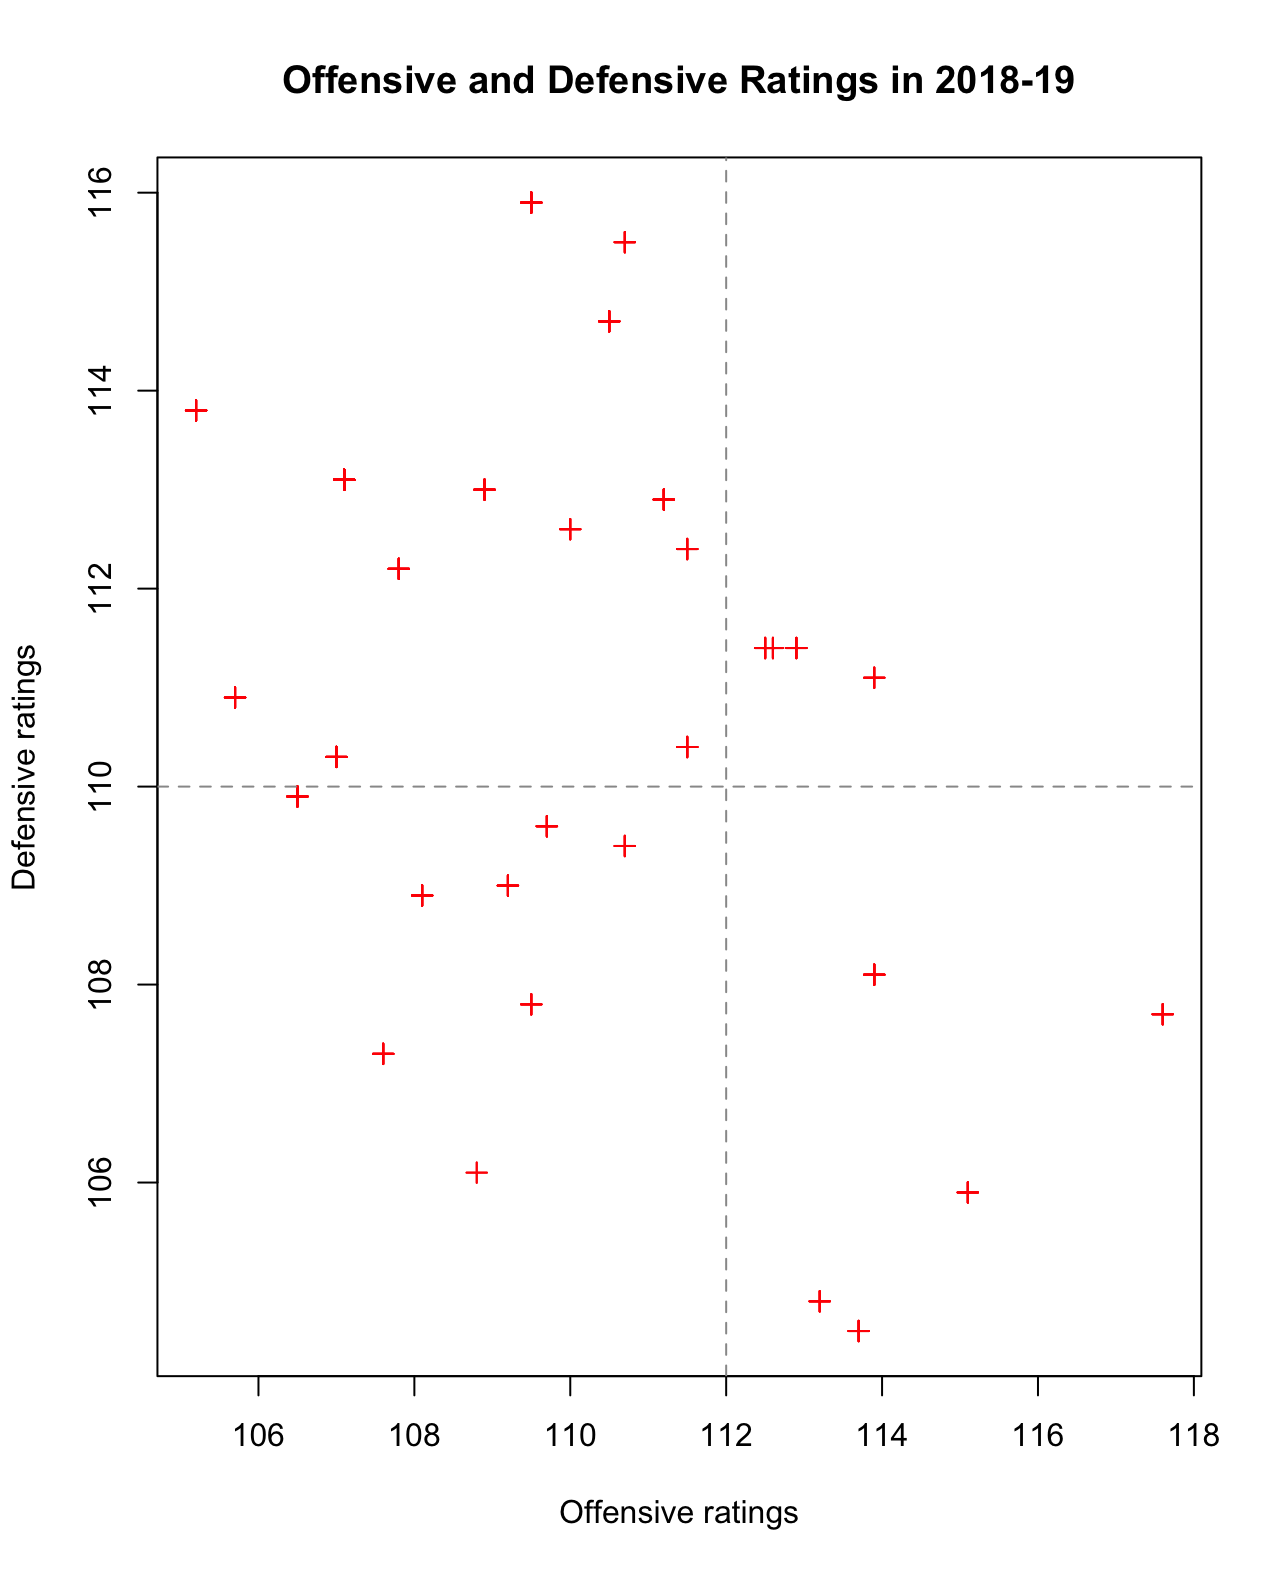
\includegraphics[width=10cm]{ORgtDRgt.png}\label{fig:1}
			\centering
			\caption{攻击效率和防守效率}
		\end{figure}
		\item Offensive and Defensive Ratings进攻得分和防守失分率: 率代表每次控球的得分(失分),进攻得分率和防守失分率是根据每100次控球的总得分或者对手球队得分。根据分别考虑进攻得分和防守失分可以全面的评判一个球队的能力和长处,而不是将目标只局限于得分高低。下图展示了2018-19赛季中顶级30个球队得分率和失分率的分布图。下边的球队防守能力更强,因为对方球队的得分较低;右边的球队进攻能力很强,因为进攻得分很高。 如果只单纯根据Offensive Rating和 Defensive Rating来衡量一个球队的优秀程度多少有一些偏差,这时需要引入球队净得分来更全面的衡量。Net Rating是球队每100次进攻中得分与失分的差。用来衡量球队风格,和更全面的评判球队的表现。一个球队如果在整个赛季中净得分大于0,说明进攻性更强。当然球队的净得分和球员的表现有很大的关系。球队的净得分均值是0. 
	
		\item Pace Adjustment 进攻效率调整:一个获得100次球权的 球队,比一个获得80次进攻机会的球队多25\%的机会进行投篮,助攻,篮板等,所以当两个球队有不同的控球次数时,需要调整获得的数据。不同的控球次数来源于球队不同的进攻风格,若一个球队的步伐相对缓慢,称为有更少的进攻机会。根据调整球队进攻步伐获得更统一的衡量标准。
		
		\end{enumerate}
		
	\end{enumerate}


\noindent 将个体球员指标转化为整个球队整体球员的指标:\\按照每支球队整个赛季中各个球员在场时间将球员排序,将个体球员构建四个指标分别和上场时间相乘,将每队上场时间最长的12个球员的上述指标与上场时间相乘后的指标相加得到某球队整体球员效率,整体球员命中率,整体球员有效利用率,和整体球员得分率。\\
该计算方法的意义:
	\begin{enumerate}
		\item  由于个体球员的指标与该赛季球员的比赛时长相关,该方法以时间作为权重,对球队球员的指标进行加权求和,返回整体球队球员的指标。
		\item 一些球员通过选秀等方式会被交易到其他球队,所以要计算球员上场时间最长的12个球员,更充分可以反映球员对球队的贡献。因为这12个球员是球队中比较稳定的中流砥柱.
		\item 该计算方法也可以自动给四个指标更高的球员赋予更大的权重,因为四个指标分别是衡量球员命中率,球员效率,球员利用率以及球员有效得分率的指标,指标值越高的球员上场时间可能更长,而指标值较低的球员的上场时间会相对较短,所以时长作为权重,可以很好的平衡球员之间的效率。
		
	\end{enumerate}
最终得到的指标分别为球队胜率W/L\%(因变量),比分差距MOV/A,球队攻击效率ORtg/A, 球队防守效率DRtg/A,球队净得分差NRtg/A, 球队实际命中率Team\_TSR, 球队球员有效得分率Team\_eFGP,球队有效利用率Team\_USR,球队整体球员效率Team\_PER,球队控球次数Team\_Poss。
	
	\section{描述性统计分析}
	下面进行指标的统计描述分析:主要是对上部分构造的球队数据进行统计描述。


%插入图片
\begin{enumerate}
	\item {\bfseries 球队胜率 球队胜率W/L\%}胜率的分布图如左图\ref{fig:2},可以看出胜率是近似的正态分布,轻微右偏,是轻尾的正态分布函数。根据右图\ref{fig:3}可知,在设定置信水平为95\%的情况下,正态分布和实际数据的点共同在蓝色置信带中,并且围绕在正态分布直线的两侧;
	\begin{figure}[h]
		
		\begin{subfigure}{0.5\textwidth}
			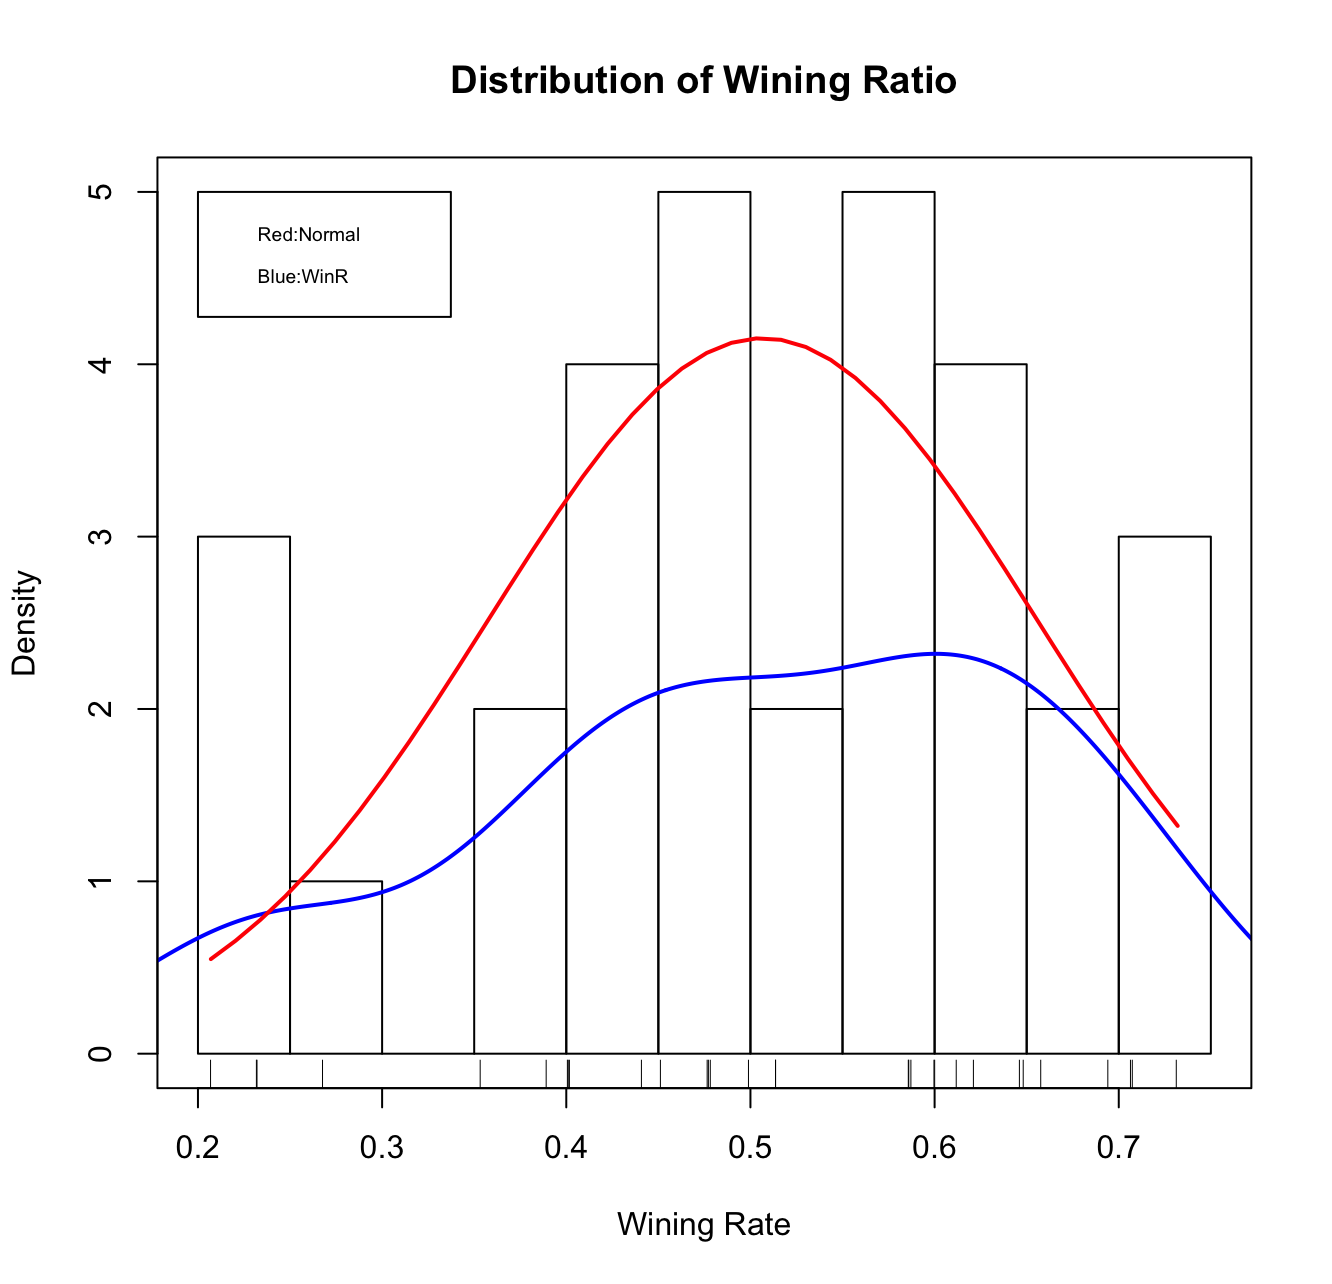
\includegraphics[width=0.9\linewidth, height=5cm]{distribution.png} 
			\caption{胜率分布图}
			\label{fig:2}
		\end{subfigure}
		\begin{subfigure}{0.5\textwidth}
			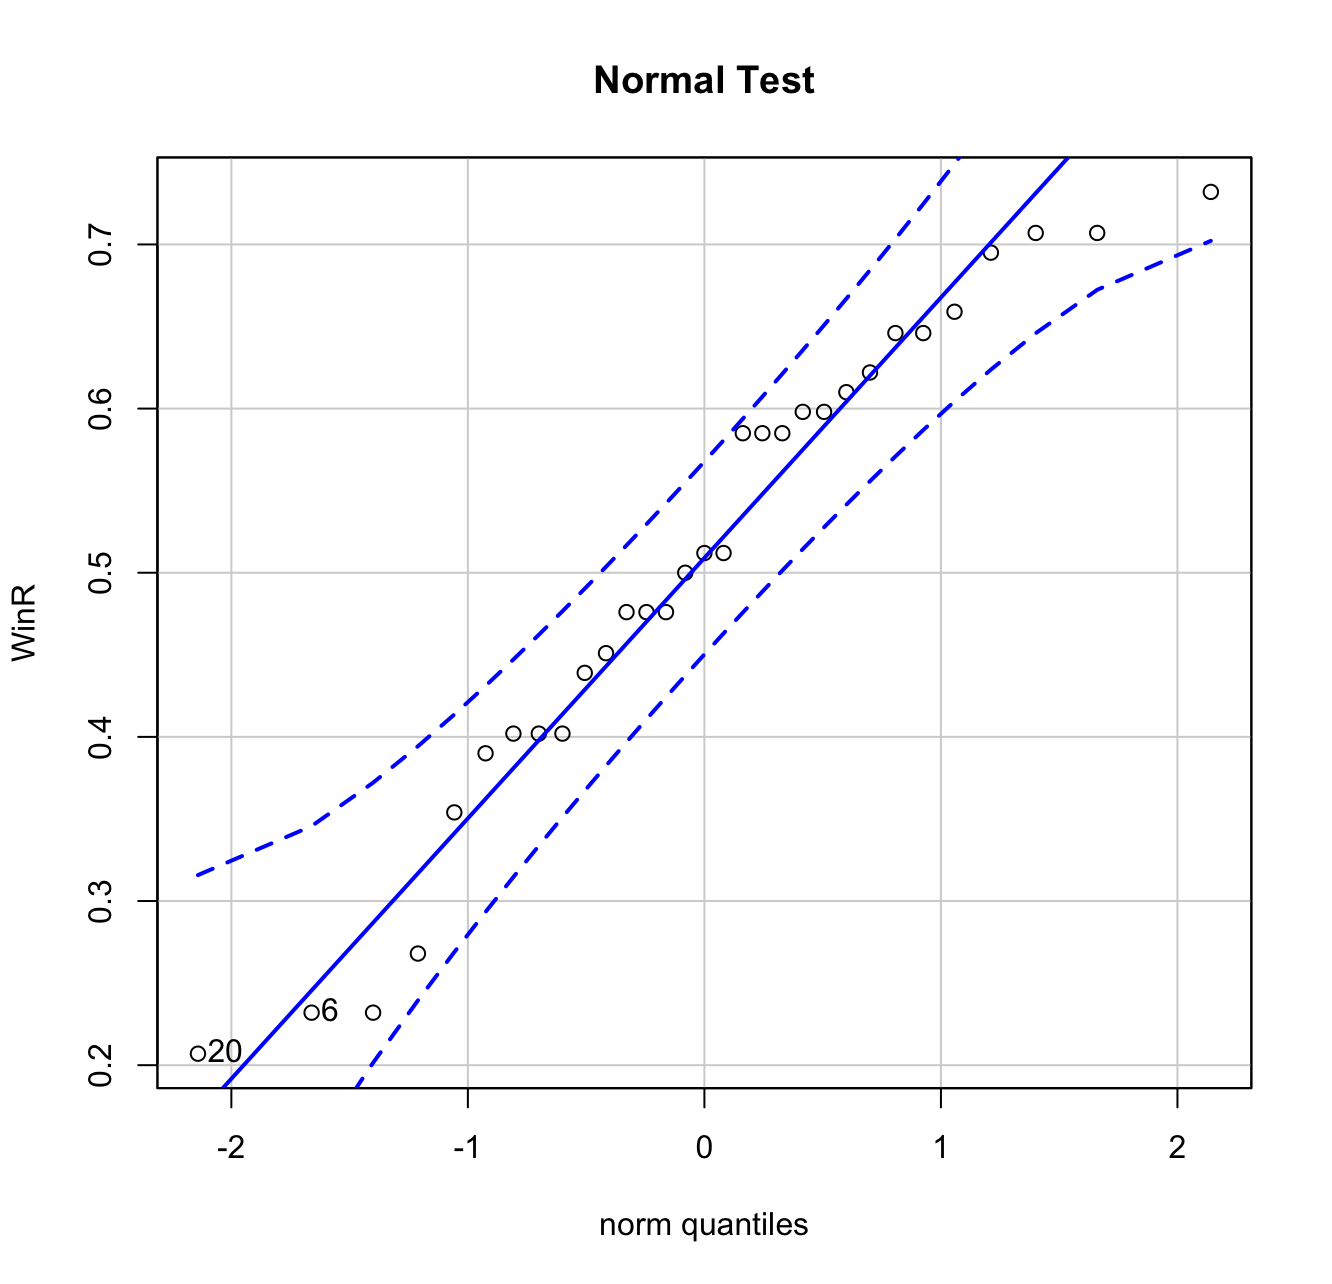
\includegraphics[width=0.9\linewidth, height=5cm]{NormTest}
			\caption{正态检验图}
			\label{fig:3}
		\end{subfigure}
	\caption{胜率统计描述图}
	\end{figure}
	在建模中希望数据服从近似正态分布,所以应对数据进行近一步正态性检验。
	利用Shapino-Wilks正态性检验,零假设为该样本符合正态分布,可看到如下表 $p=0.14>0.1$ ,可知在置信度为95\%水平下无法拒绝原假设,不能推翻样本的正太性假设。

	%正太性检验结果
	\begin{table}[h!]
			\begin{tabular}{|c|c|}
			\hline
			\multicolumn{2}{|c|}{Shapiro-Wilk normality test} \\
			\hline
			\multicolumn{2}{|c|}{ data:  data\$`W/L\%`} \\
			\hline
			W = 0.94857 &p-value = 0.1425\\
			\hline
		\end{tabular}
	\centering
	\label{4}
	\caption{正太性检验}
	\end{table}

%第二个变量	
	
\begin{figure}[h!]
	
	\begin{subfigure}{0.5\textwidth}
		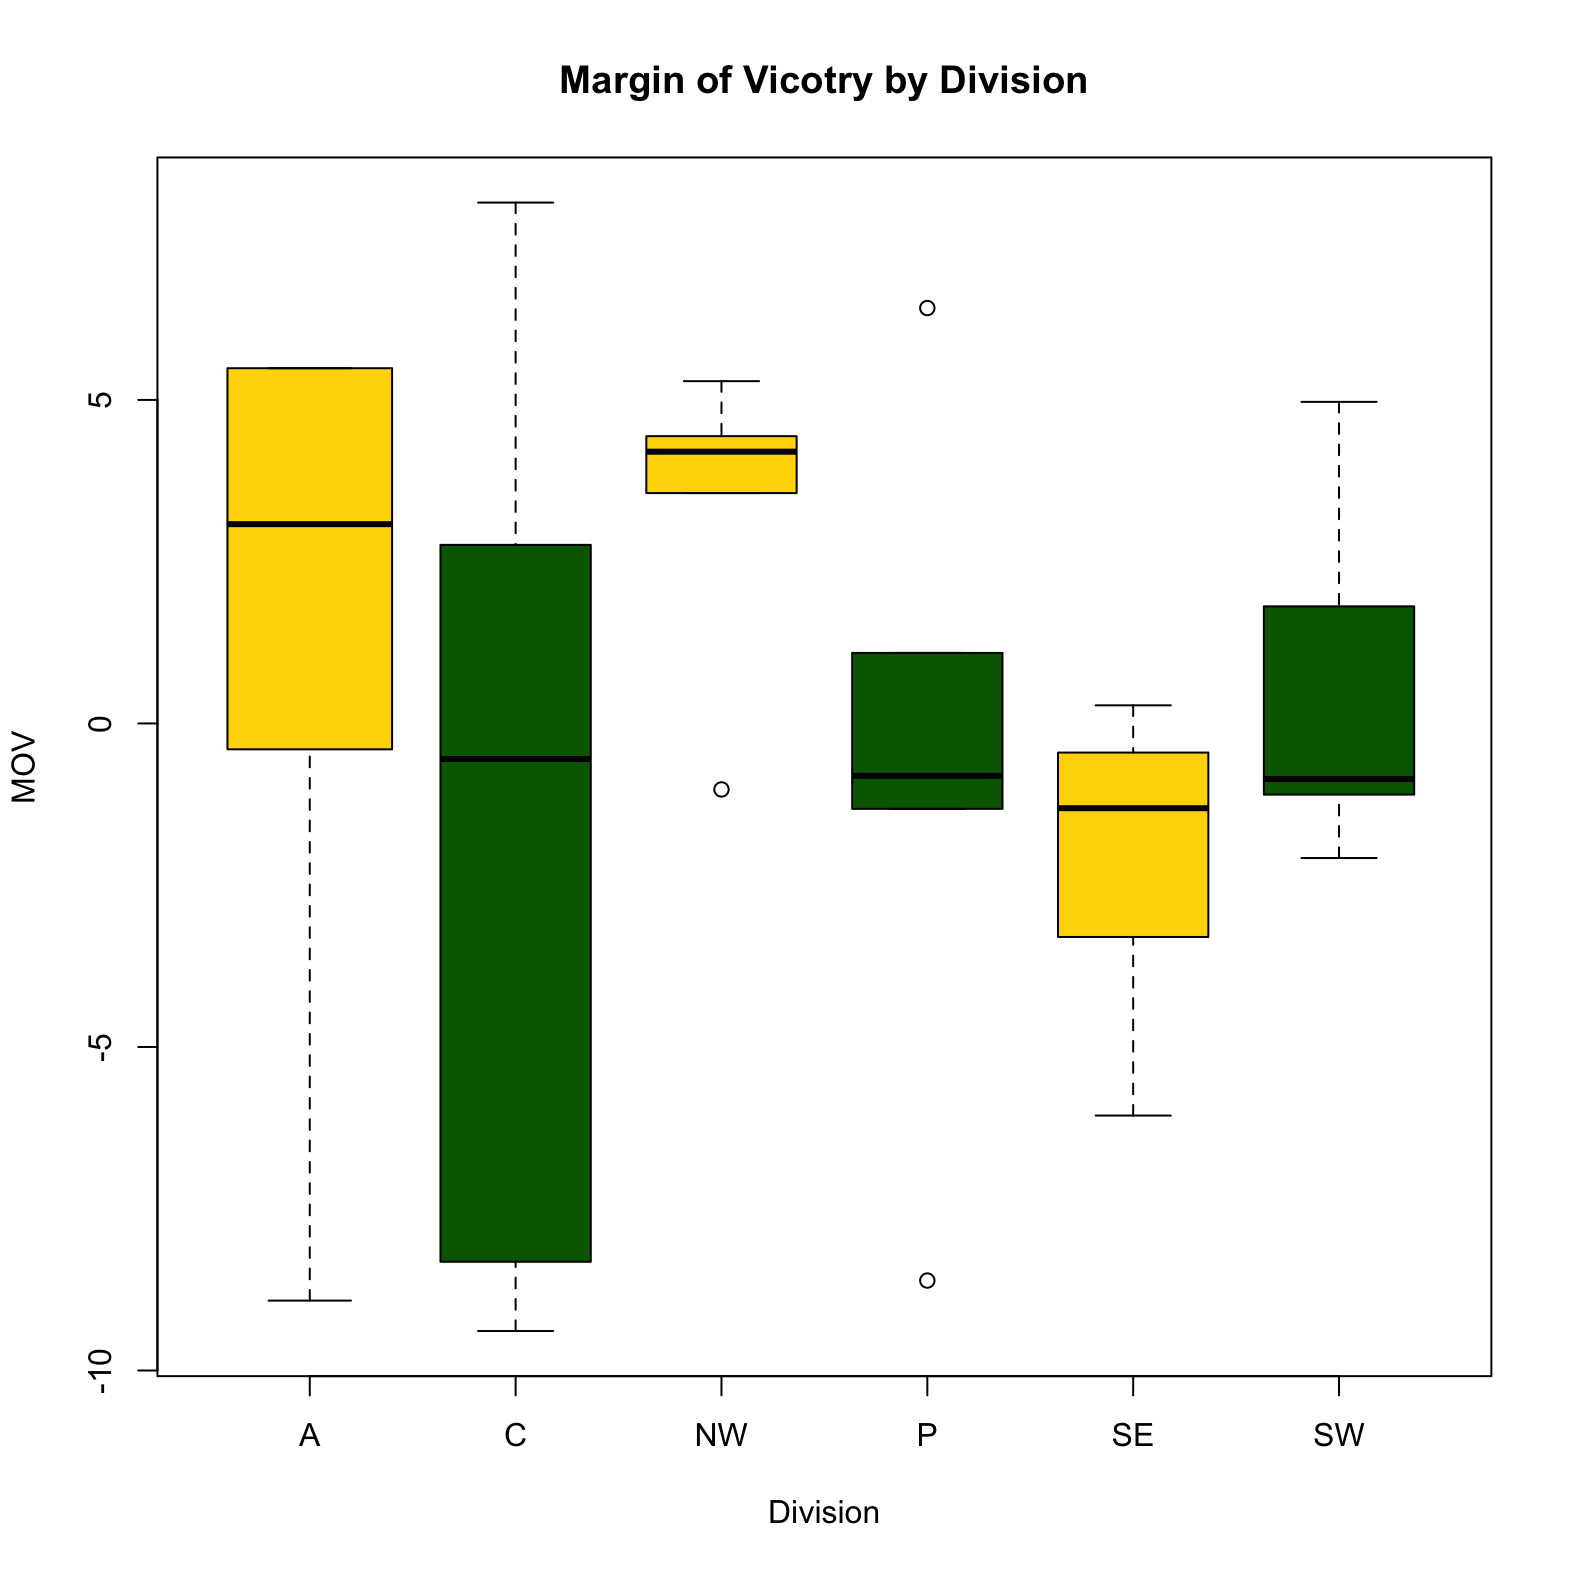
\includegraphics[width=0.9\linewidth, height=5cm]{MOVbp.png} 
		\caption{MOV的箱线图}
		\label{fig:4}
	\end{subfigure}
	\begin{subfigure}{0.5\textwidth}
		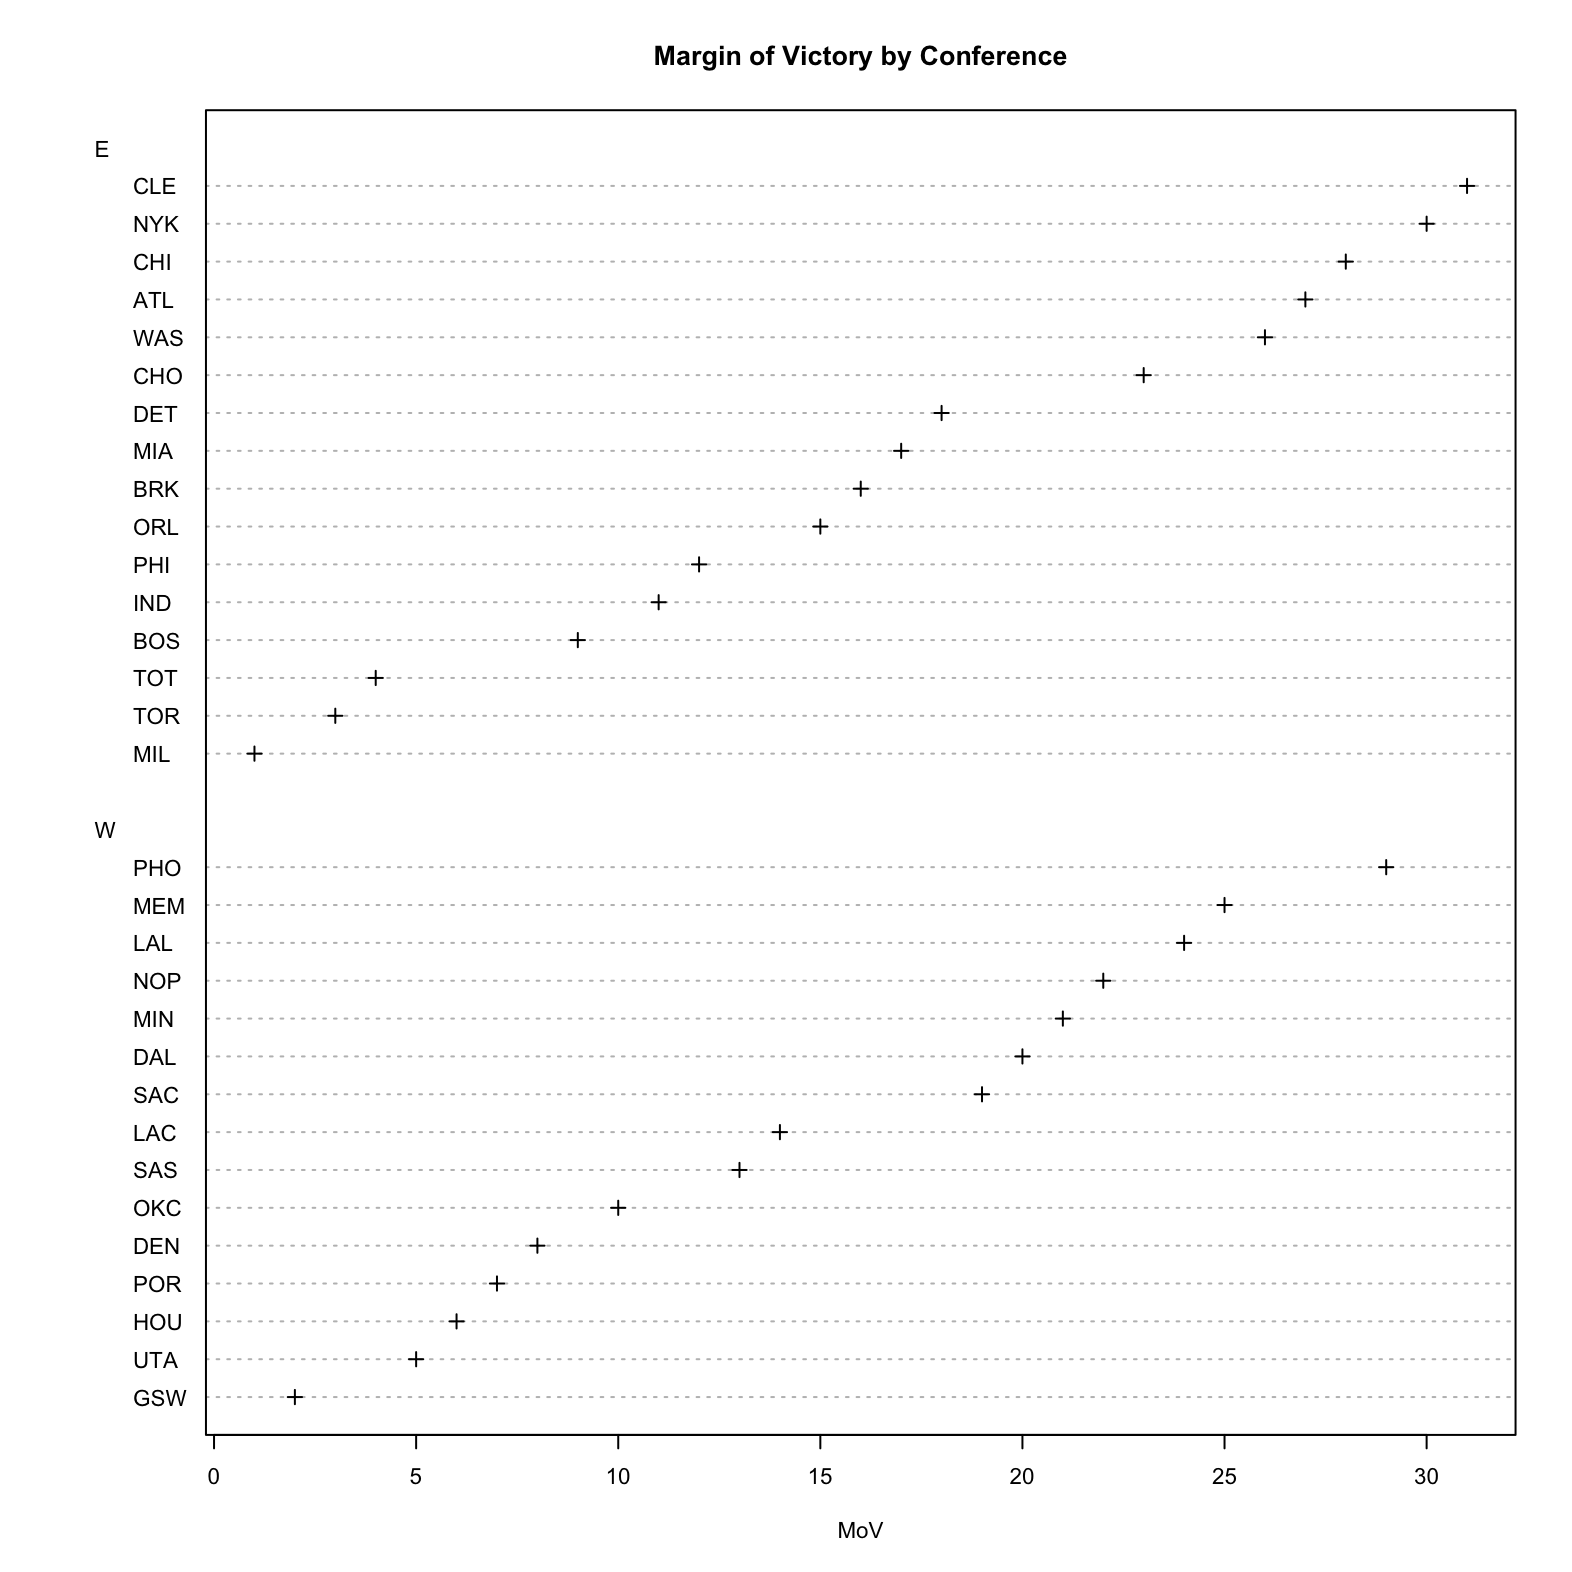
\includegraphics[width=0.9\linewidth, height=5cm]{Movdotp.png}
		\caption{MOV的散点图}
		\label{fig:5}
	\end{subfigure}
\caption{比分差距统计描述}
\end{figure}
	\item  {\bfseries 比分差距MOV/A的描述性分析:}左图\ref{fig:4}详细描绘了每个地区的比分差距变量的分布情况,其中比分差距变量分布最离散的是中部地区,涵盖了比分差距变量的最大值和最小值,西北地区的比分差距变量离散程度最小,数据最集中。亚特兰大地区和西北地区的球队比分差距变量基本位正,说明这些地区的球队实力很强;右图\ref{fig:5}详细列出了东部地区和西部地区所有队伍的比分差距的排名情况,其中比分差距最高的球队是东部地区的克利夫兰骑士队,比分差距最低的队伍是东部地区的密尔沃基雄鹿队。
%第三个变量

\item {\bfseries 进攻效率ORtg/A的描述性分析:  }左图\ref{fig:6} 详细描绘了每个地区的进攻效率变量的分布情况,右图\ref{fig:7} 详细列出了东部地区和西部地区所有队伍的比分差距的排名情况,中部地区和东南部地区的球队进攻效率相对较低,其中太平洋地区的进攻效率较为离散,根据进攻效率可以看出球队的风格差异;右图详细列出了东部地区和西部地区所有队伍的进攻效率的排名情况,其中东部地区进攻效率相较西部地区更为优秀一些,东部地区进攻效率最高的球队是纽约尼克斯,这说明该球队的风格更偏向进攻。
\begin{figure}[h!]
	
	\begin{subfigure}{0.5\textwidth}
		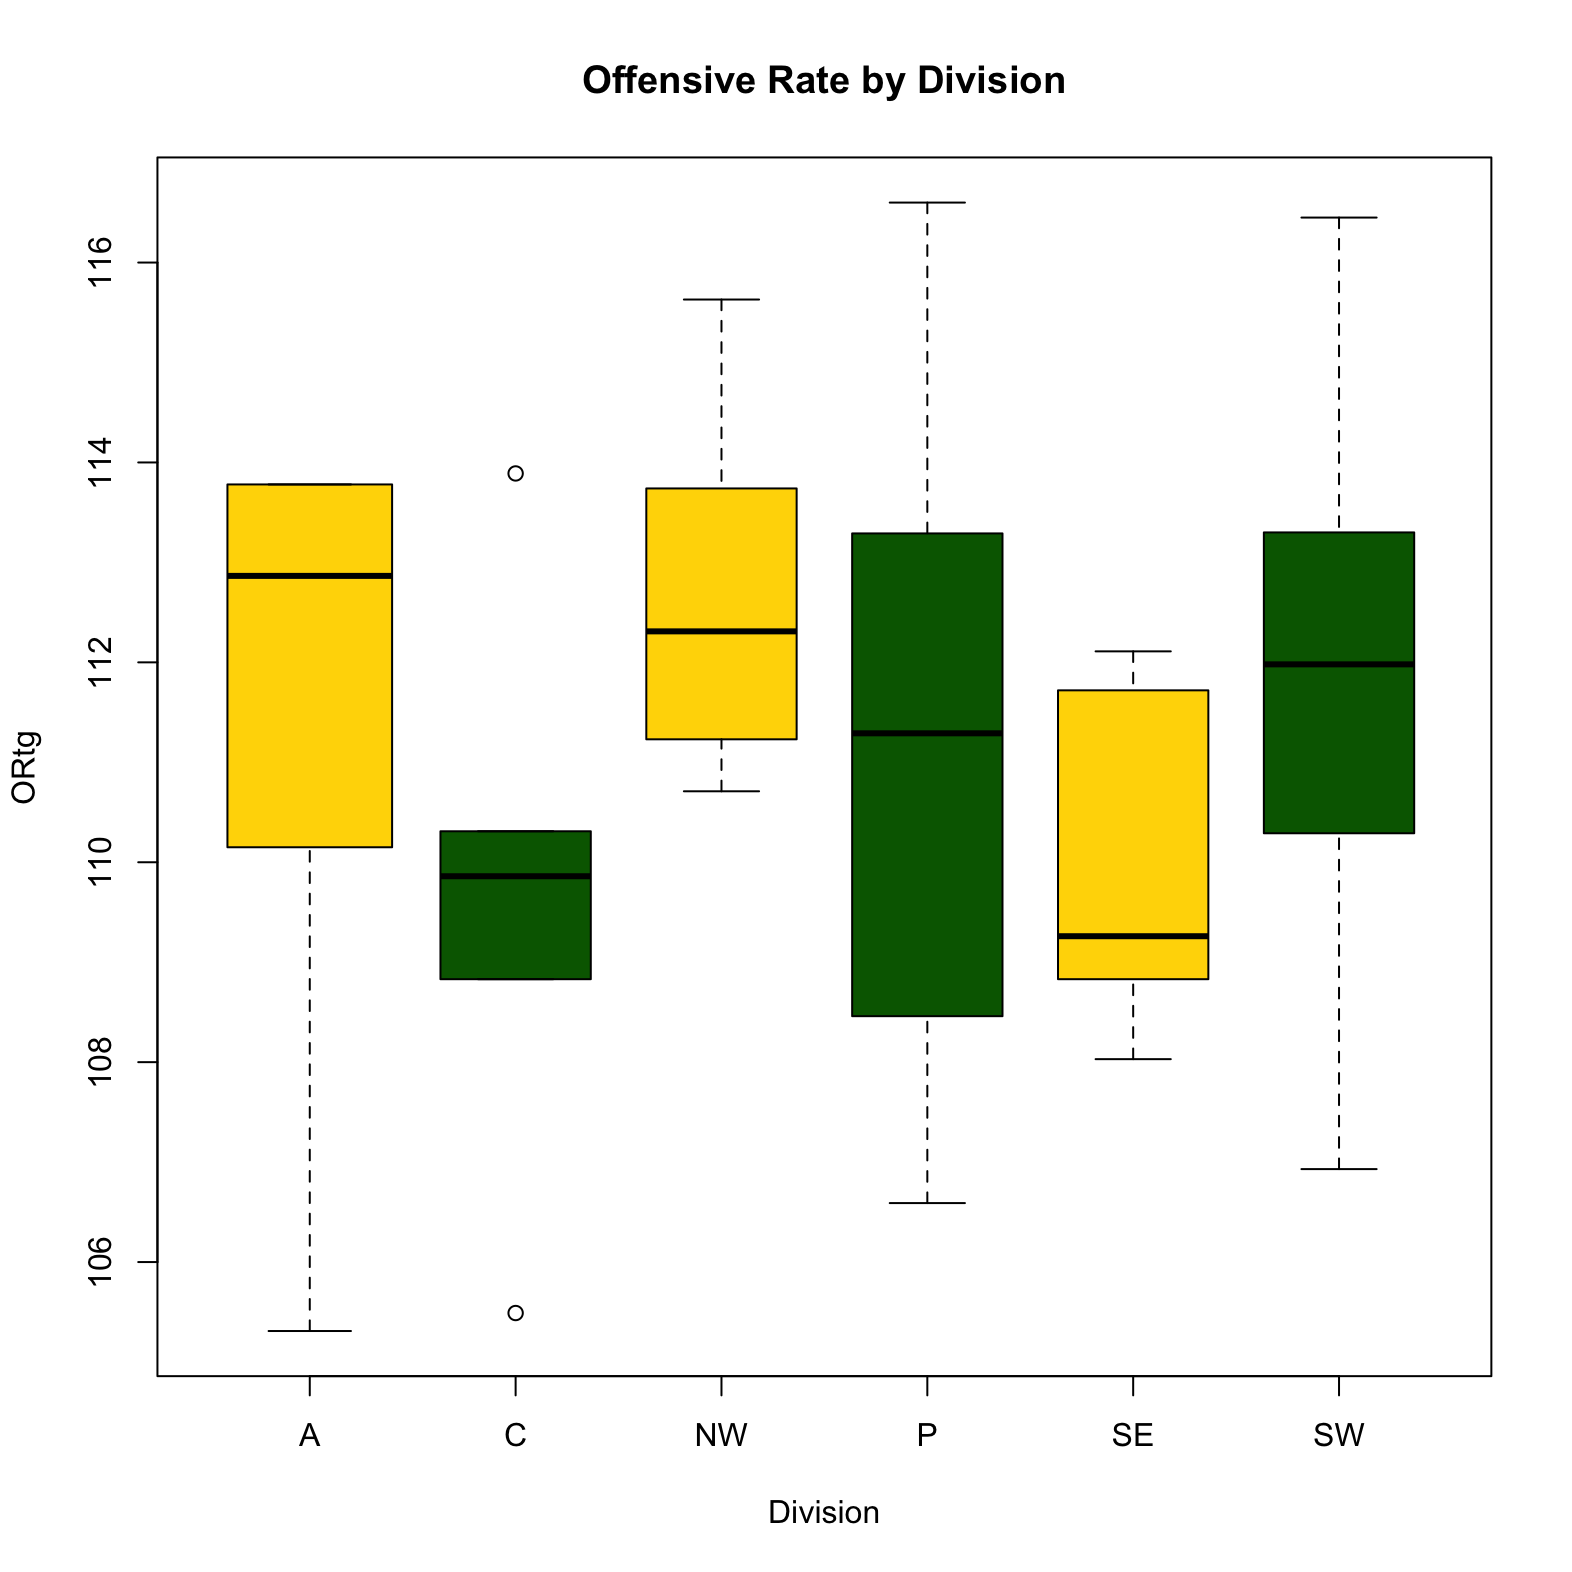
\includegraphics[width=0.9\linewidth, height=5cm]{ORgbp.png} 
		\caption{进攻效率箱线图}
		\label{fig:6}
	\end{subfigure}
	\begin{subfigure}{0.5\textwidth}
		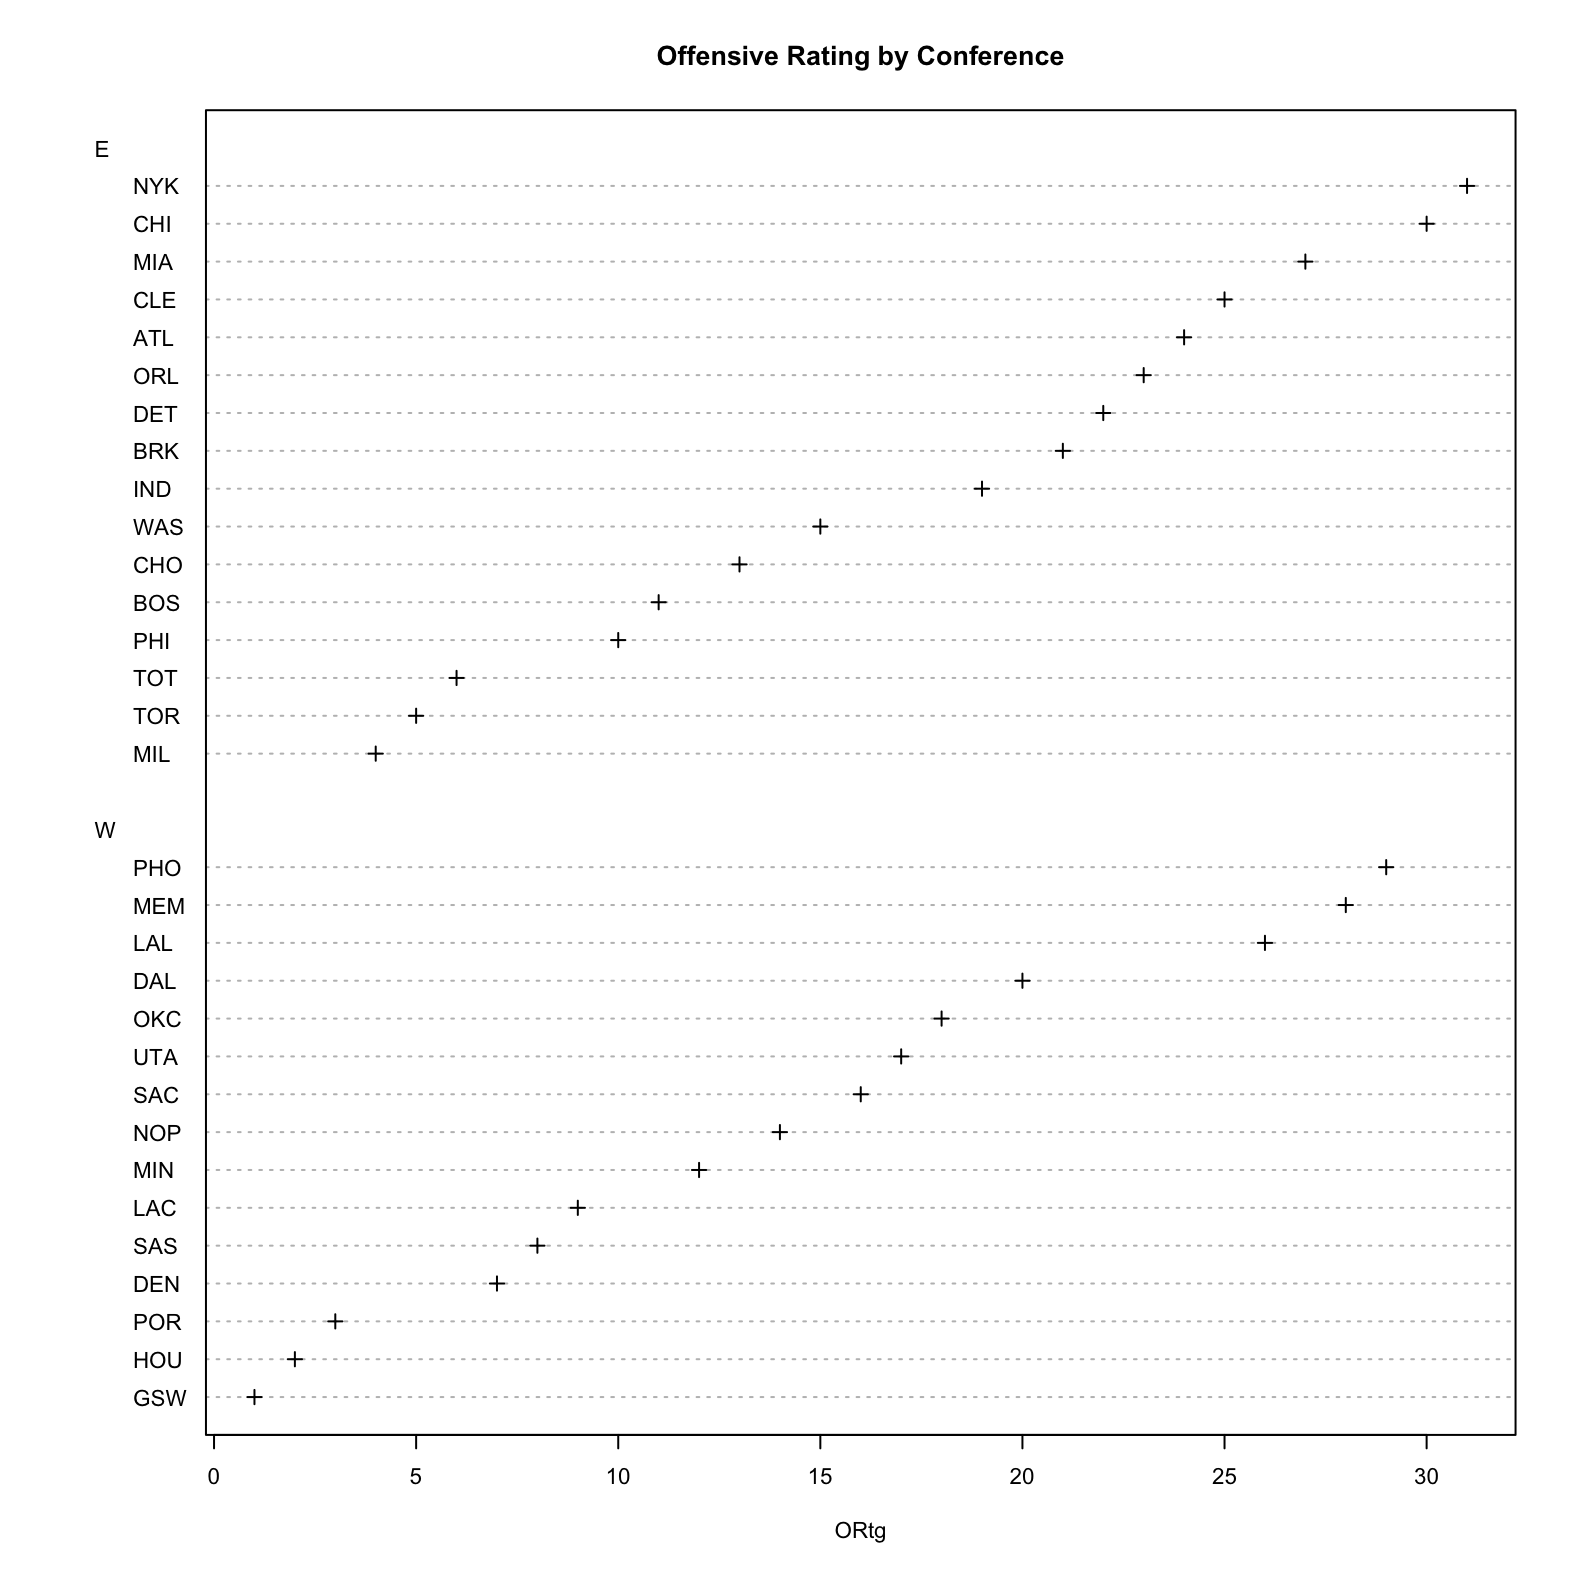
\includegraphics[width=0.9\linewidth, height=5cm]{ORtgdotp.png}
		\caption{进攻效率散点图}
		\label{fig:7}
	\end{subfigure}
	\caption{进攻效率统计描述}
\end{figure}


%第四个变量
\item {\bfseries 球员效率Team\_PER的描述统计}左图\ref{fig:8} 详细描绘了每个地区的球队的球员效率率变量的分布情况,西北部地区和西南部地区的球队的球员效率率指标分布较为集中,且这些地区的球员效率很高,即中位数是所有地区中最高的,上四分位数和下四分位数也是最高的,亚特兰大地区和东南部地区的球队球员效率变量分布较为离散;右图\ref{fig:9} 详细列出了东部地区和西部地区所有队伍球员效率变量的排名情况,东部地区的亚特兰大老鹰队球员效率最高,东部地区的费城76人队的球员效率最低。
\begin{figure}[h!]
	
	\begin{subfigure}{0.5\textwidth}
		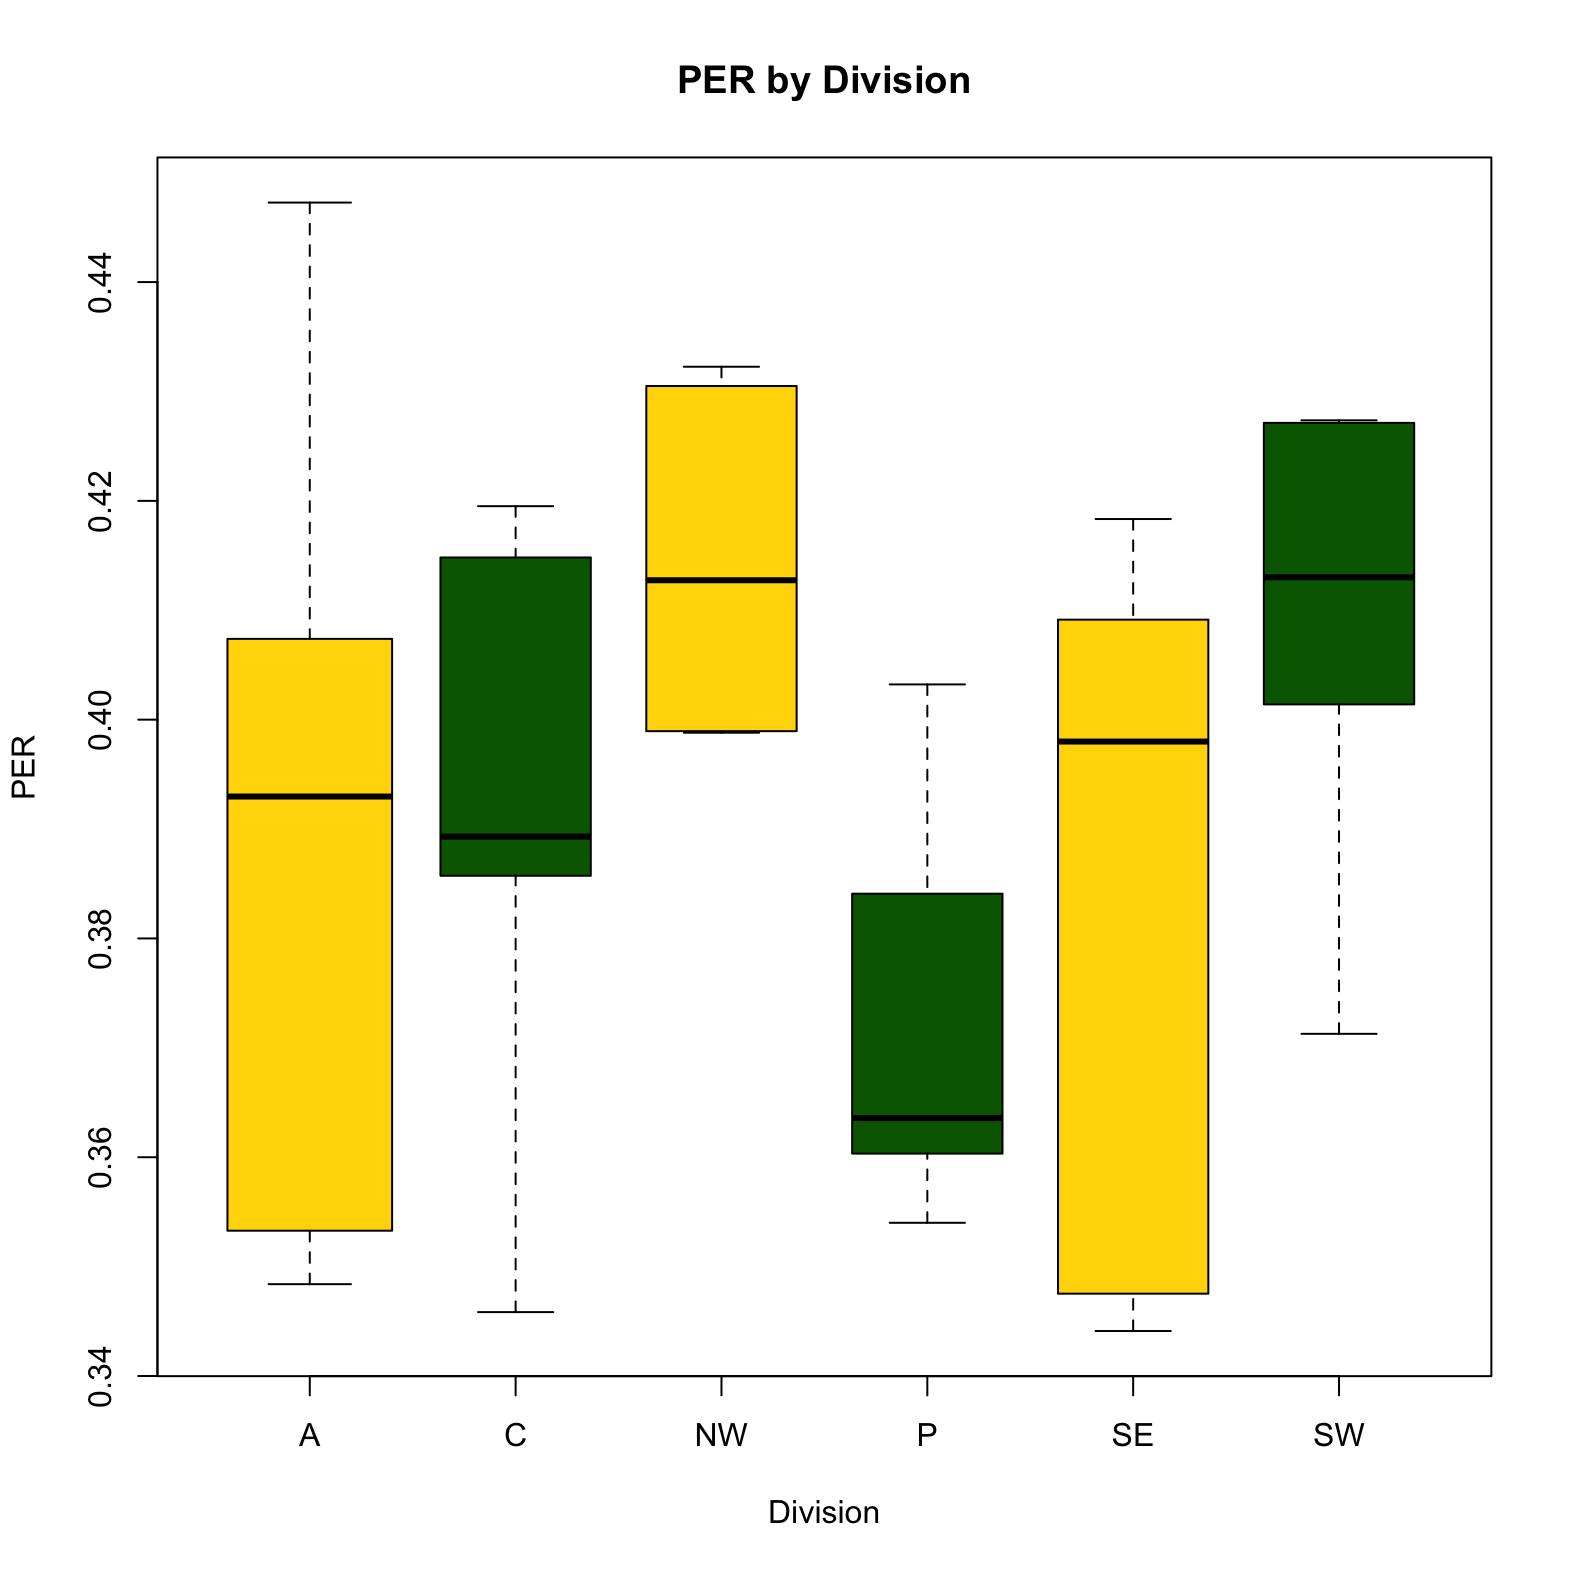
\includegraphics[width=0.9\linewidth, height=5cm]{PERbp.png} 
		\caption{球员效率箱线图}
		\label{fig:8}
	\end{subfigure}
	\begin{subfigure}{0.5\textwidth}
		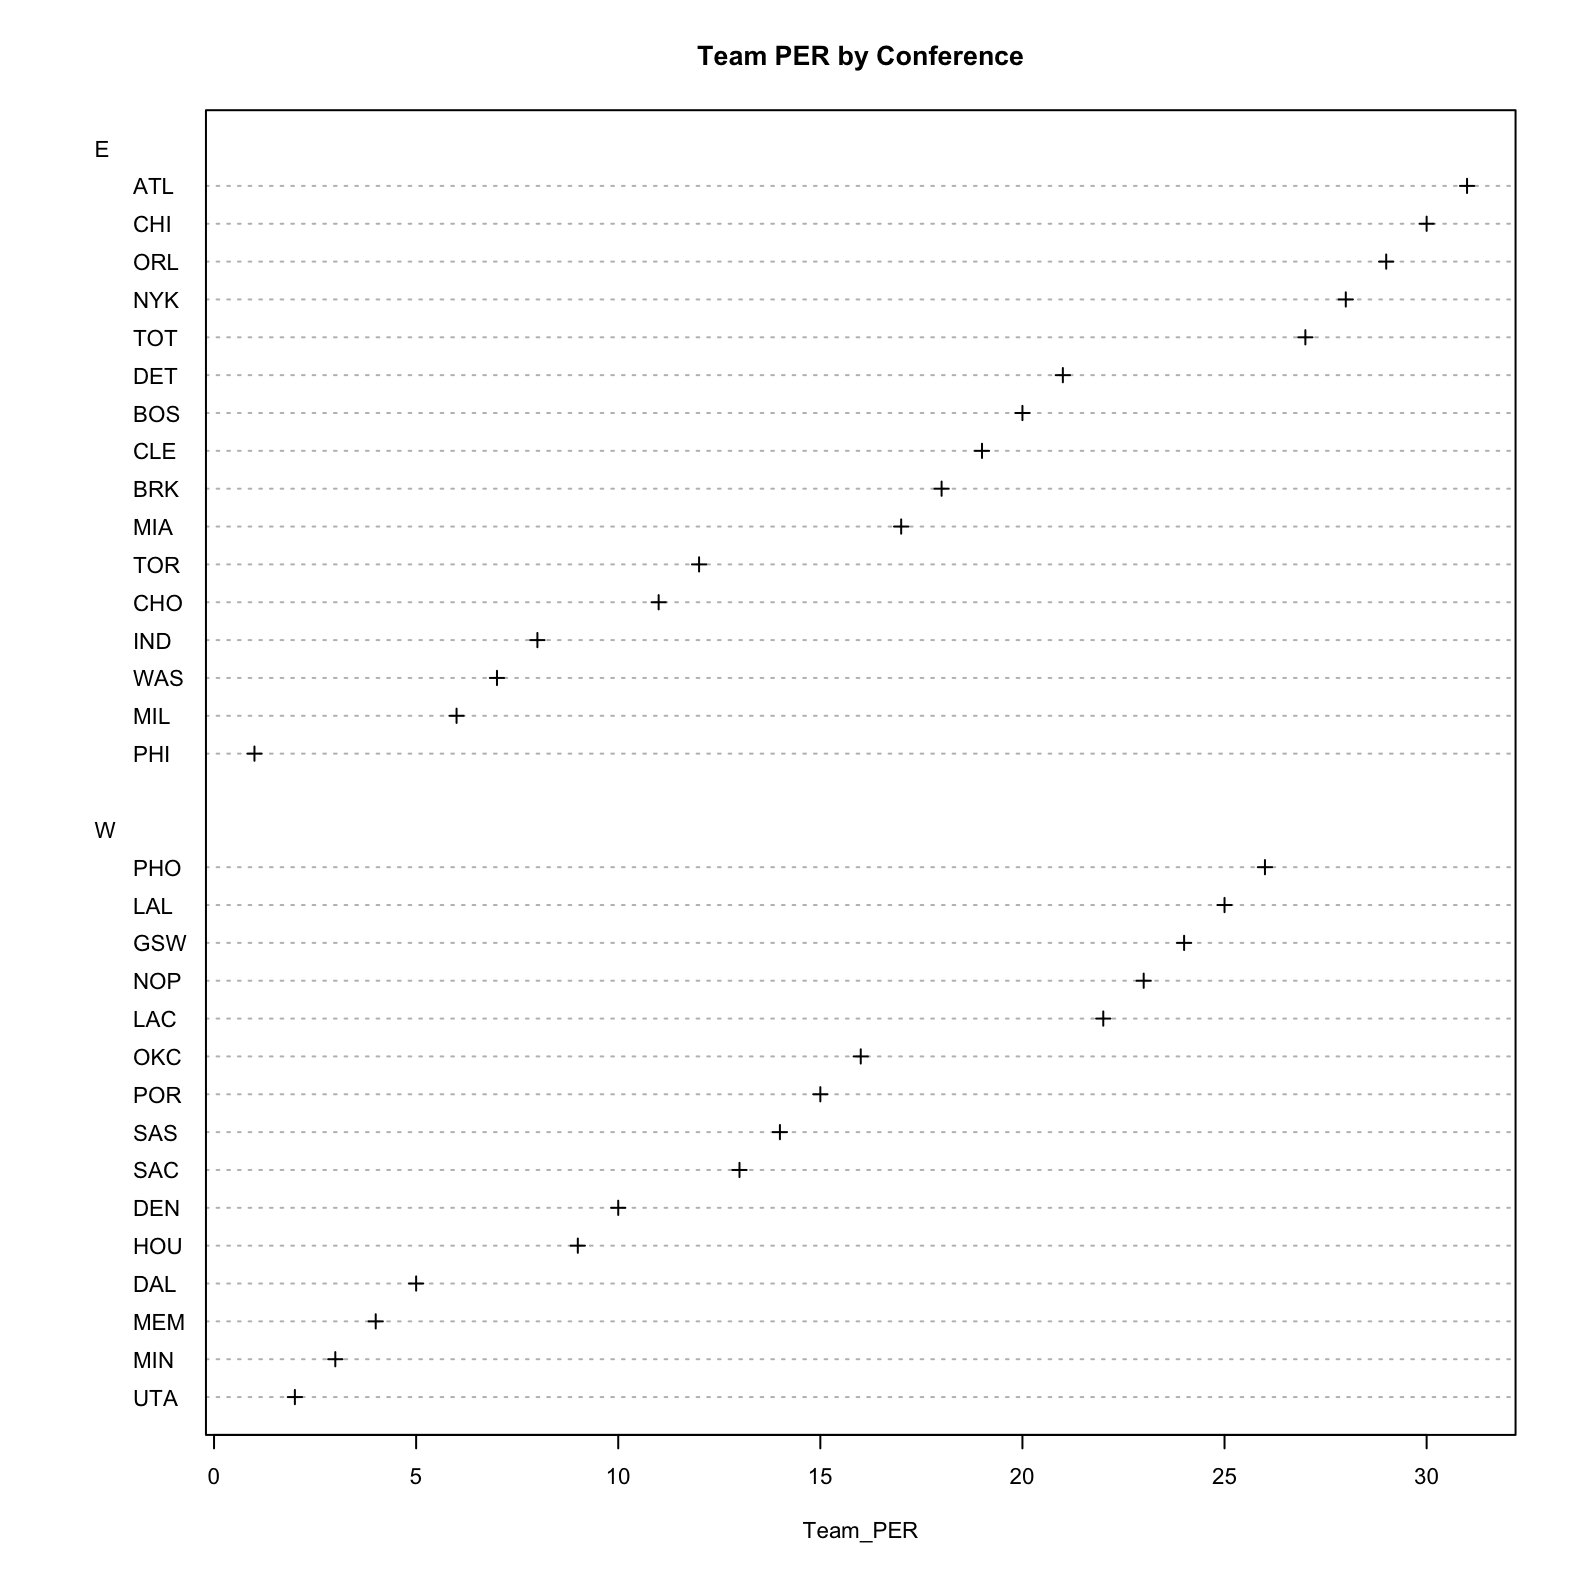
\includegraphics[width=0.9\linewidth, height=5cm]{PERdotp.png}
		\caption{球员效率散点图}
		\label{fig:9}
	\end{subfigure}
	\caption{球员效率统计描述}
\end{figure}

%第五个变量
\newpage
\item {\bfseries 球员有效得分率 Team\_eFGP的统计描述}左图\ref{fig:10}详细描绘了每个地区的球队的球员有效得分率的分布情况,可以看出各个地区球队球员有效得分率的中间水平都在0.4附近,其中太平洋地区的球队球员的有效得分率中位数最低,西南地区球队的球员有效得分率分布最离散;右图\ref{fig:11}详细列出了东部地区和西部地区所有队伍球员效率变量的排名情况,东部地区的球员有效得分率最高的球队是CHI,NYK,TOT,芝加哥公牛,多伦多猛龙队,纽约尼克斯队。东部球队的球员有效得分率相对西部球队较高。

\begin{figure}[h!]
	
	\begin{subfigure}{0.5\textwidth}
		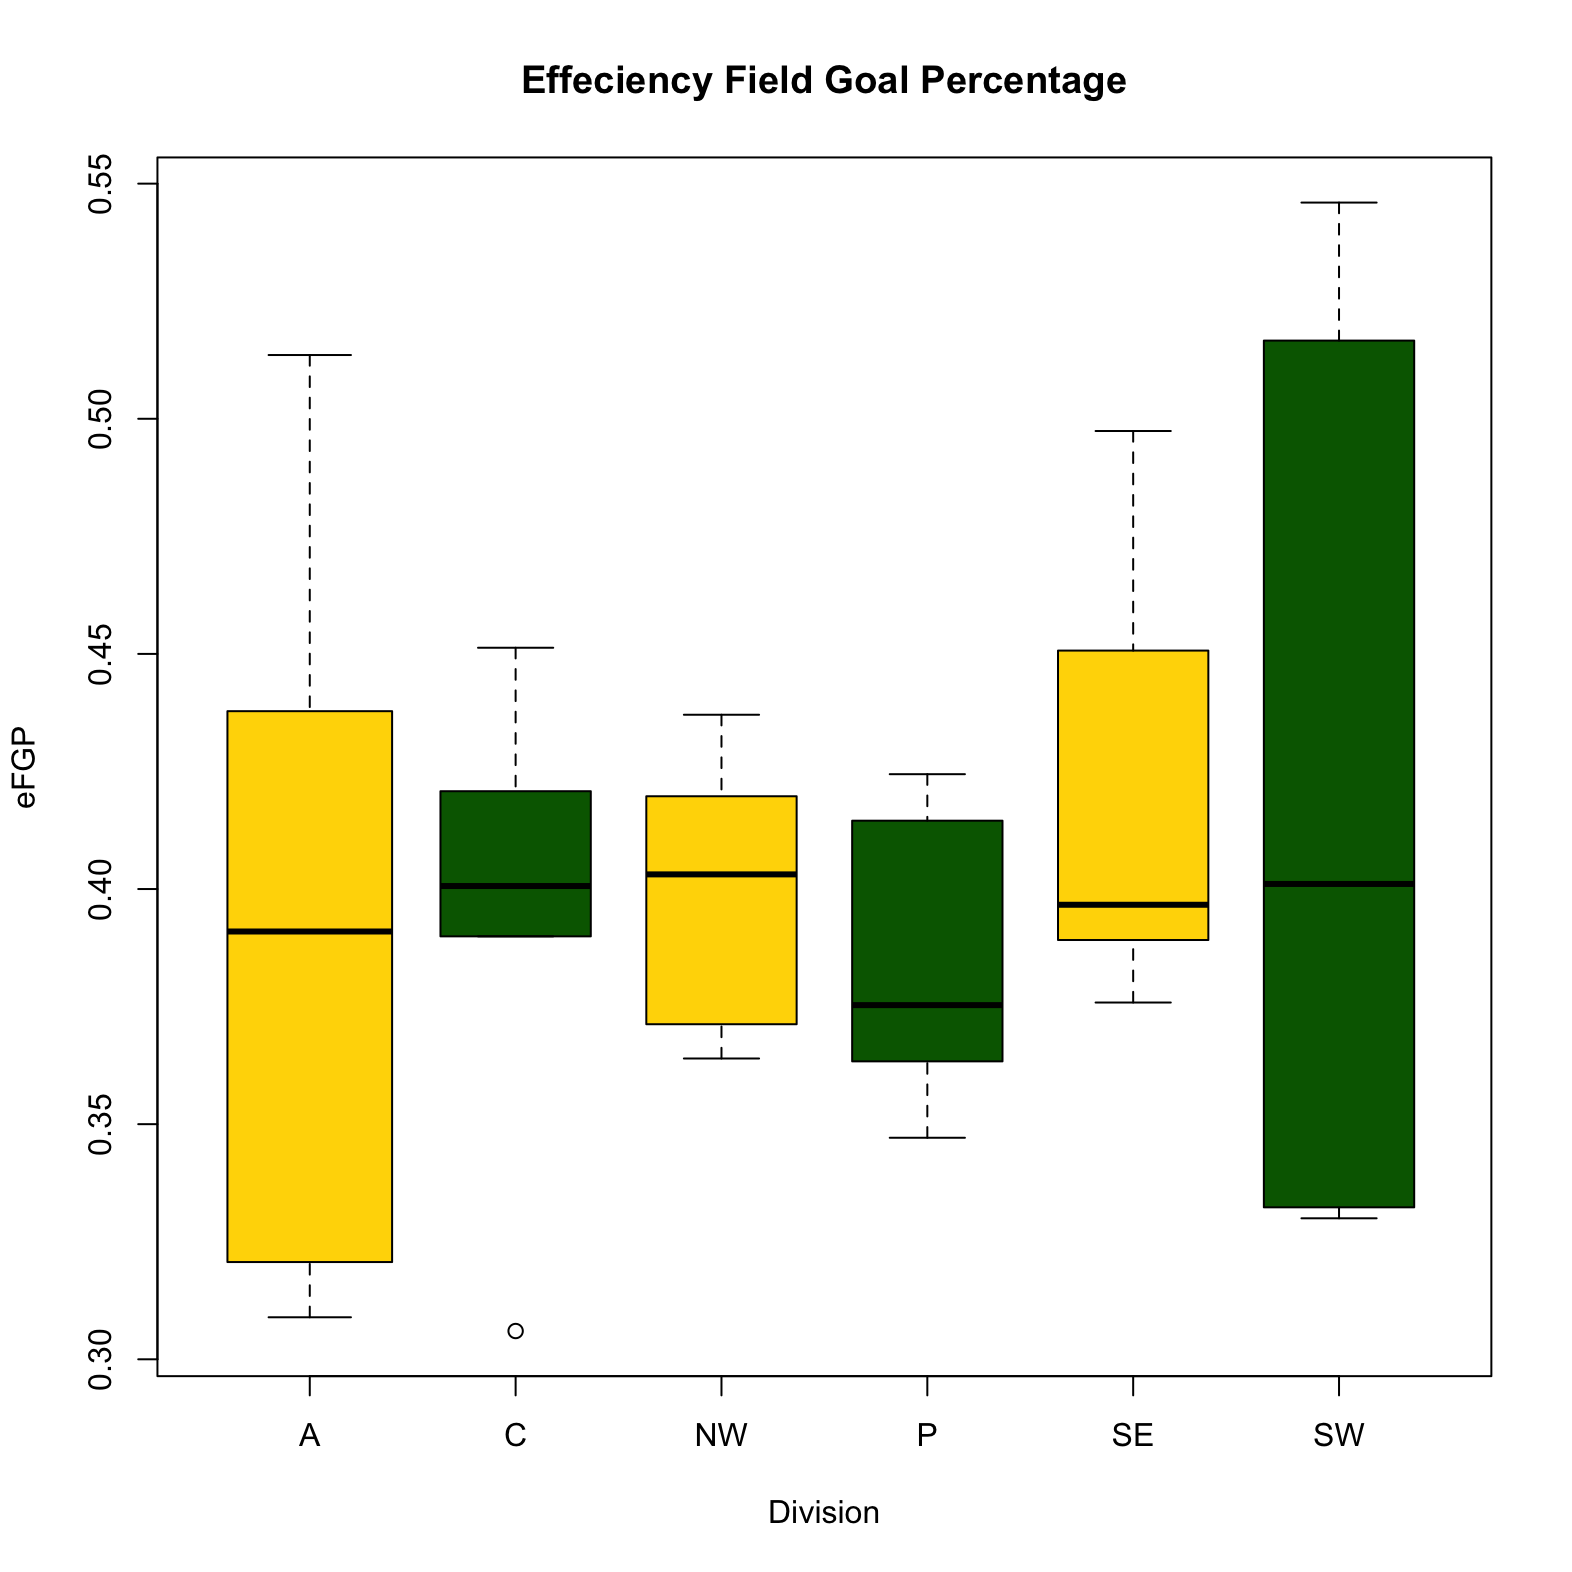
\includegraphics[width=0.9\linewidth, height=5cm]{eFGP.png} 
		\caption{有效得分率箱线图}
		\label{fig:10}
	\end{subfigure}
	\begin{subfigure}{0.5\textwidth}
		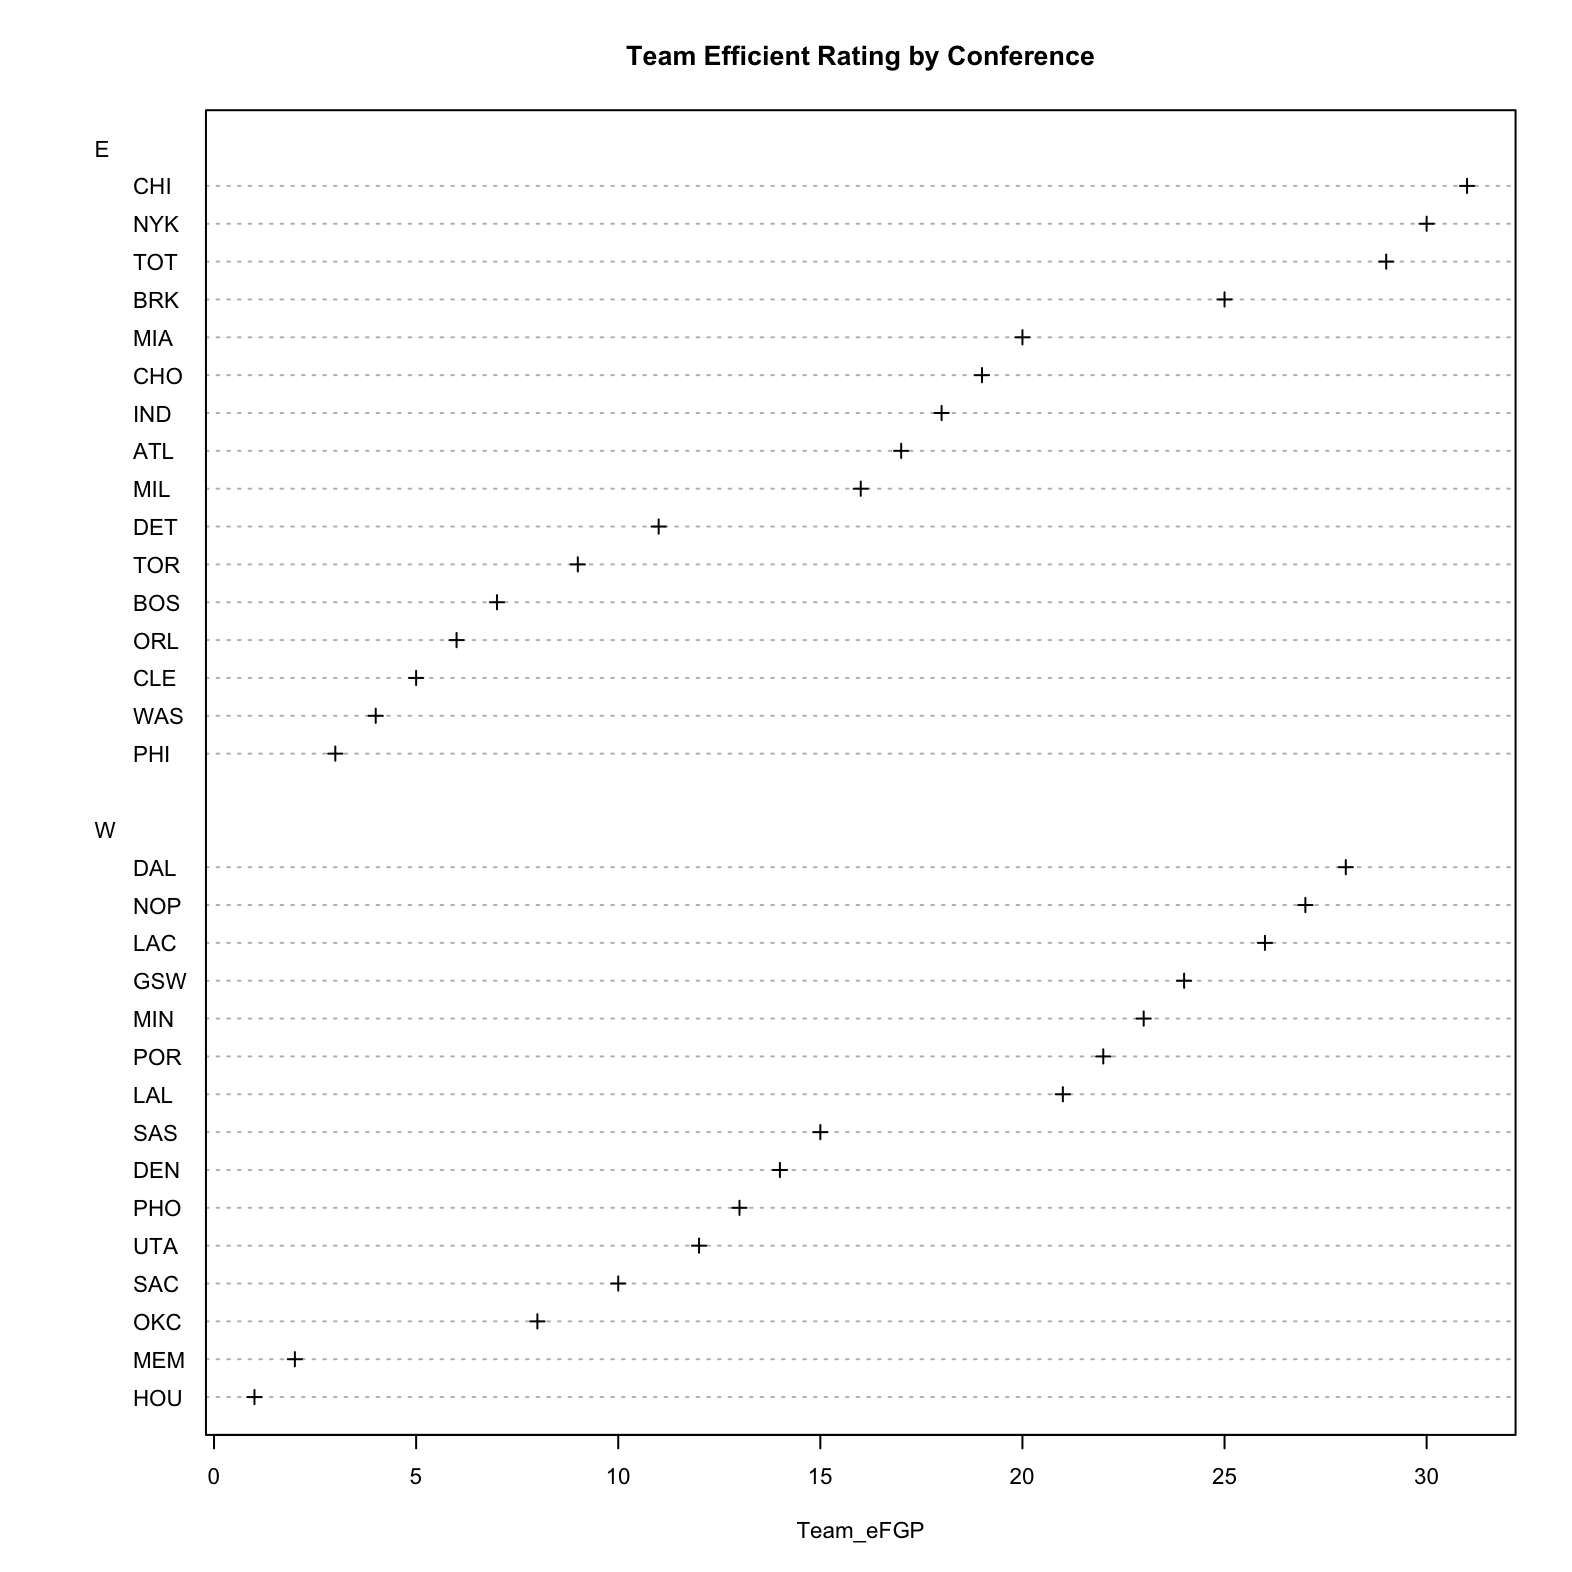
\includegraphics[width=0.9\linewidth, height=5cm]{eFGPdotp.png}
		\caption{有效得分率散点图}
		\label{fig:11}
	\end{subfigure}
	\caption{有效得分率统计描述}
\end{figure}

%第六个变量
\item {\bfseries 球队球员实际命中率Team\_TSR描述性统计分析}左图\ref{fig:12}详细描绘了每个地区的球队球员的实际命中率率的分布情况,可以看出实际命中率变量各个地区的中位数差距不大,但是亚特兰大地区和西南地区的分布差距较大,东南地区存在极端值,其他地区球队球员实际命中率的分布较为集中;右图\ref{fig:13}详细列出了东部地区和西部地区所有队伍球员的实际命中率变量的排名情况, 球员实际命中率最高的球队是西部的新奥尔良黄蜂
, 东部的纽约尼克斯和芝加哥公牛,多伦多猛龙队。

\begin{figure}[h!]
	
	\begin{subfigure}{0.5\textwidth}
		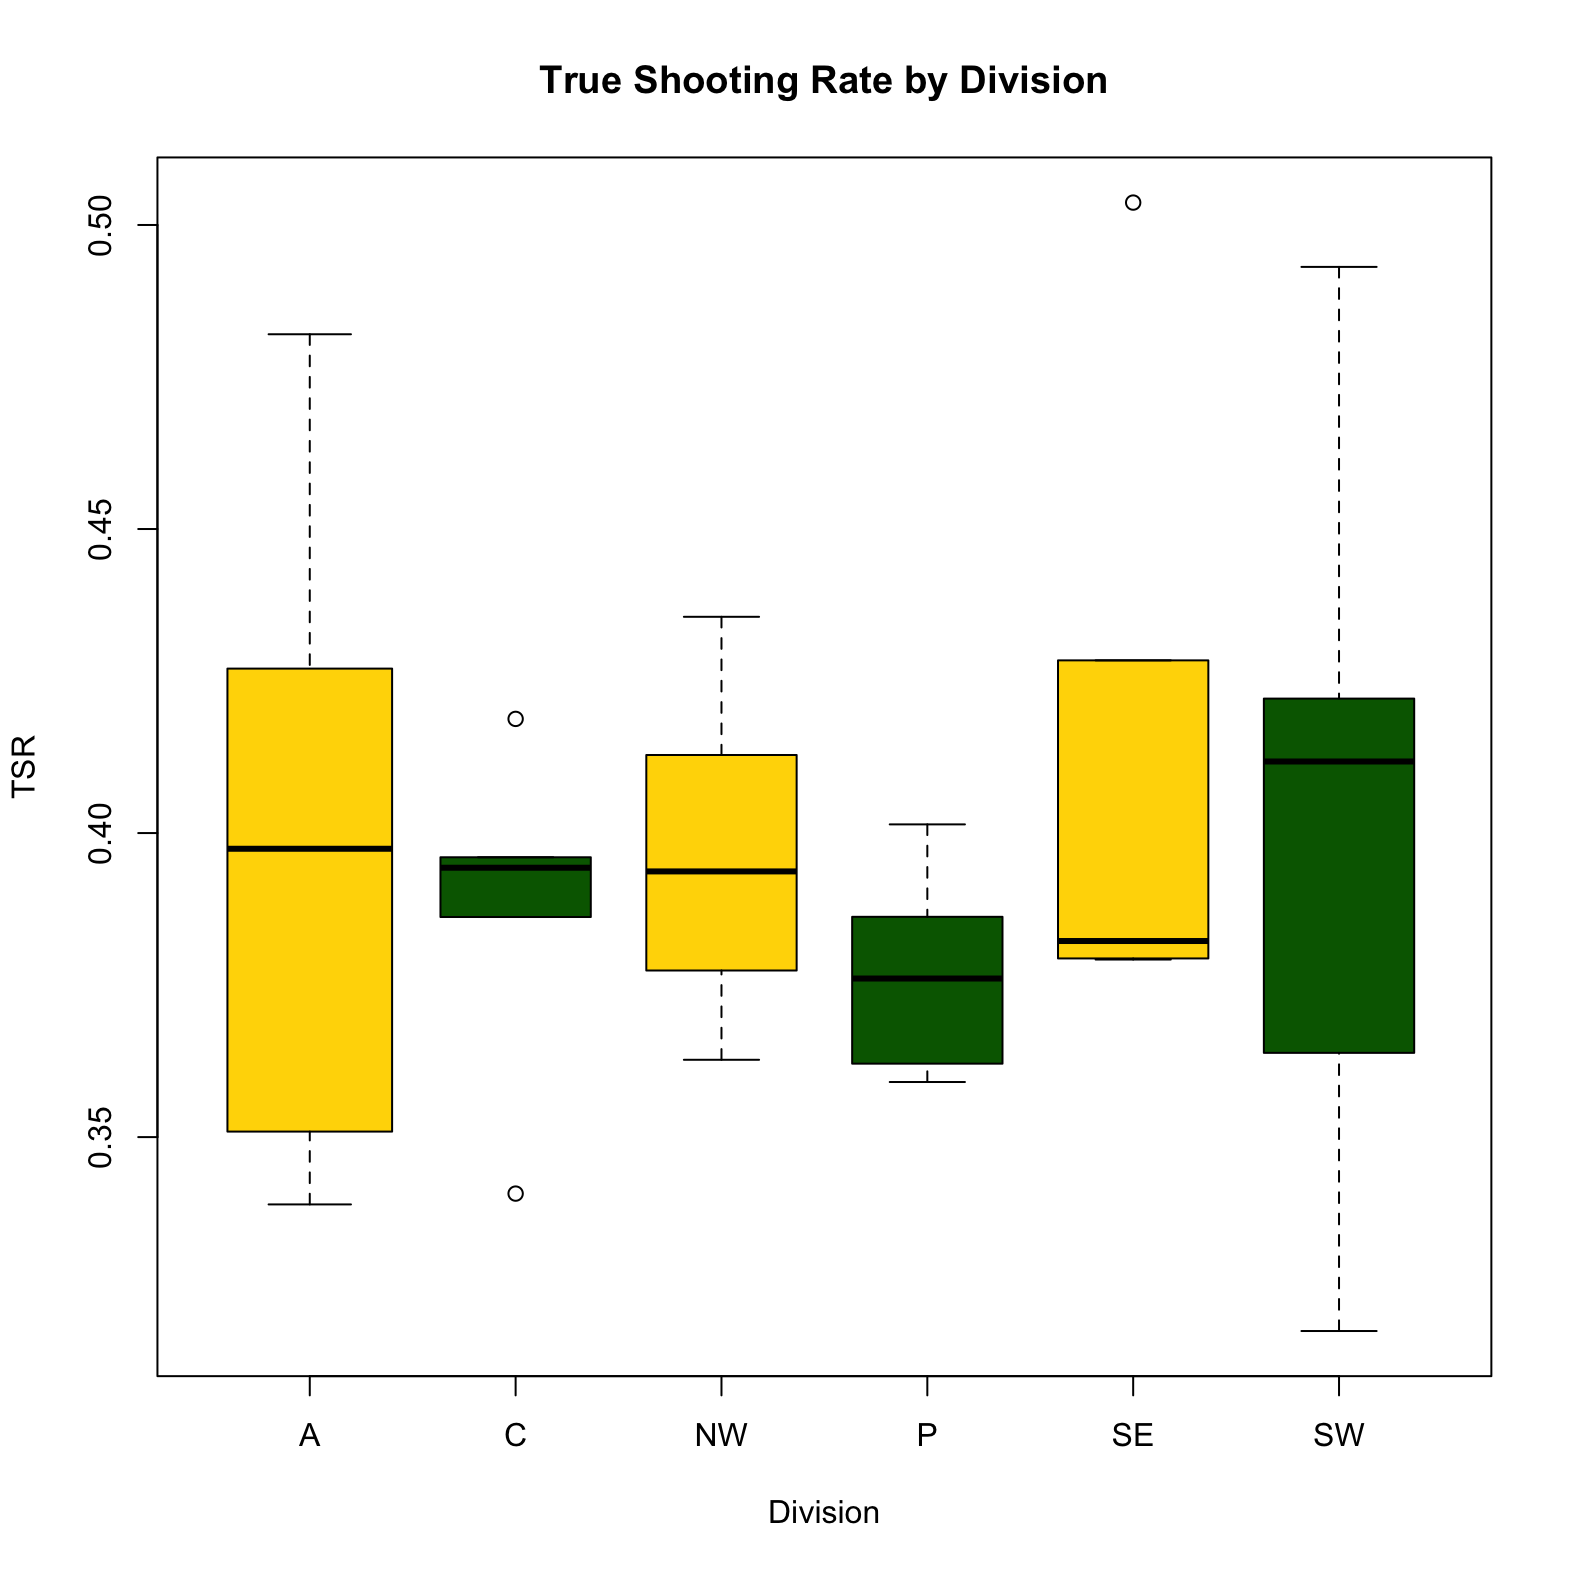
\includegraphics[width=0.9\linewidth, height=5cm]{TSRbp.png} 
		\caption{实际命中率箱线图}
		\label{fig:12}
	\end{subfigure}
	\begin{subfigure}{0.5\textwidth}
		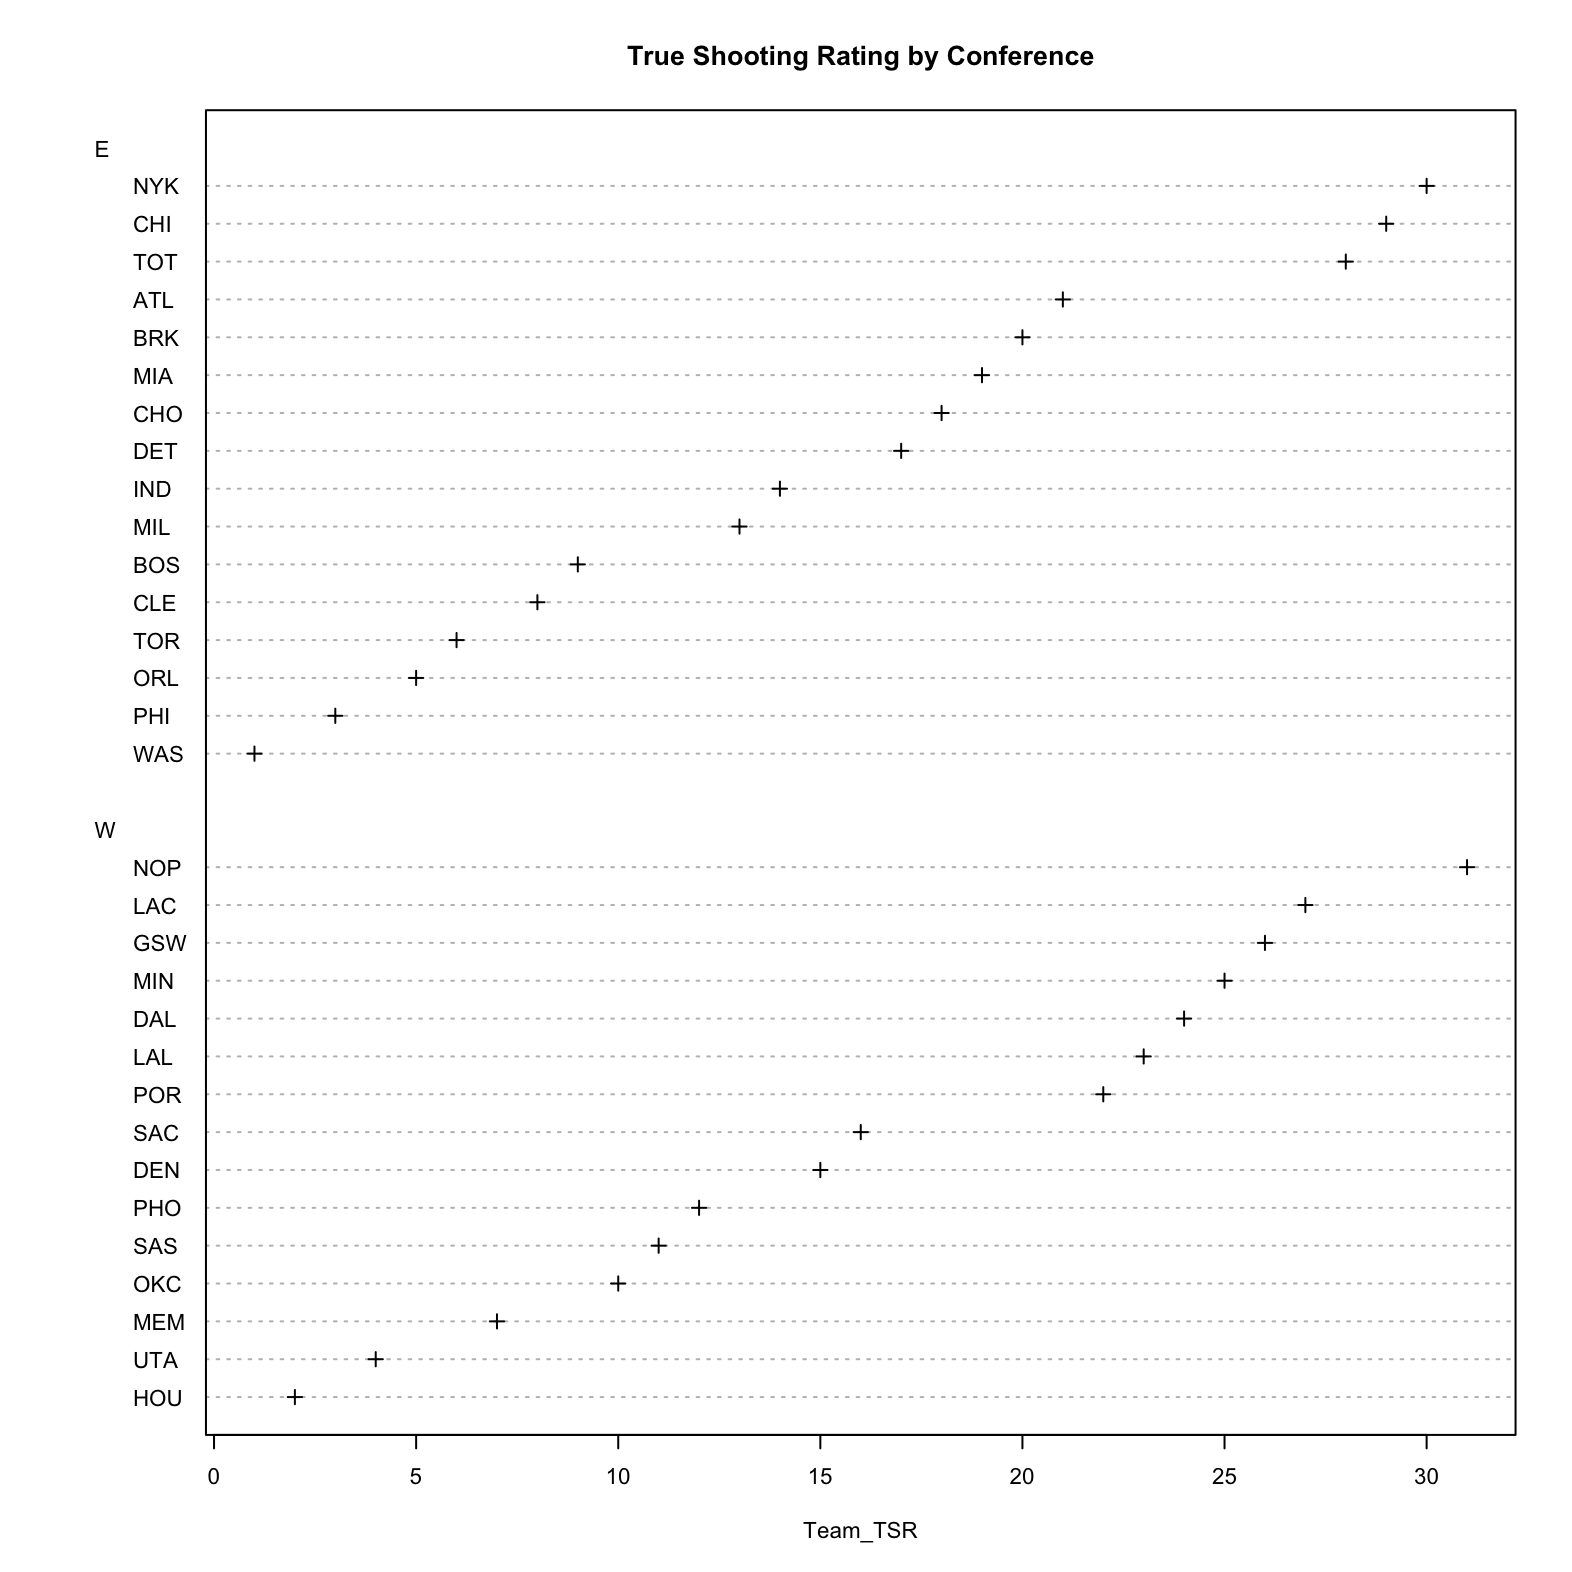
\includegraphics[width=0.9\linewidth, height=5cm]{TSRdotp.png}
		\caption{实际命中率散点图}
		\label{fig:13}
	\end{subfigure}
	\caption{实际命中率统计描述}
\end{figure}


%第7个变量
\newpage
\item {\bfseries 球队球员利用率Team\_USR的统计描述}左图\ref{fig:14}详细描绘了每个地区的球队球员利用率的分布情况,可以看出各地区的球员利用率差距较大,其中西南地区球队的球员利用率变量分布情况较离散,西北地区和东南地区的球队的球员利用率分布情况较为集中。球员利用率变量中位数最高的地区是太平洋地区; 右图\ref{fig:15}详细列出了东部地区和西部地区所有队伍球员利用率变量的排名情况,西部地区的克利夫兰骑士队拥有最高的球员利用率。
\begin{figure}[h!]
	
	\begin{subfigure}{0.5\textwidth}
		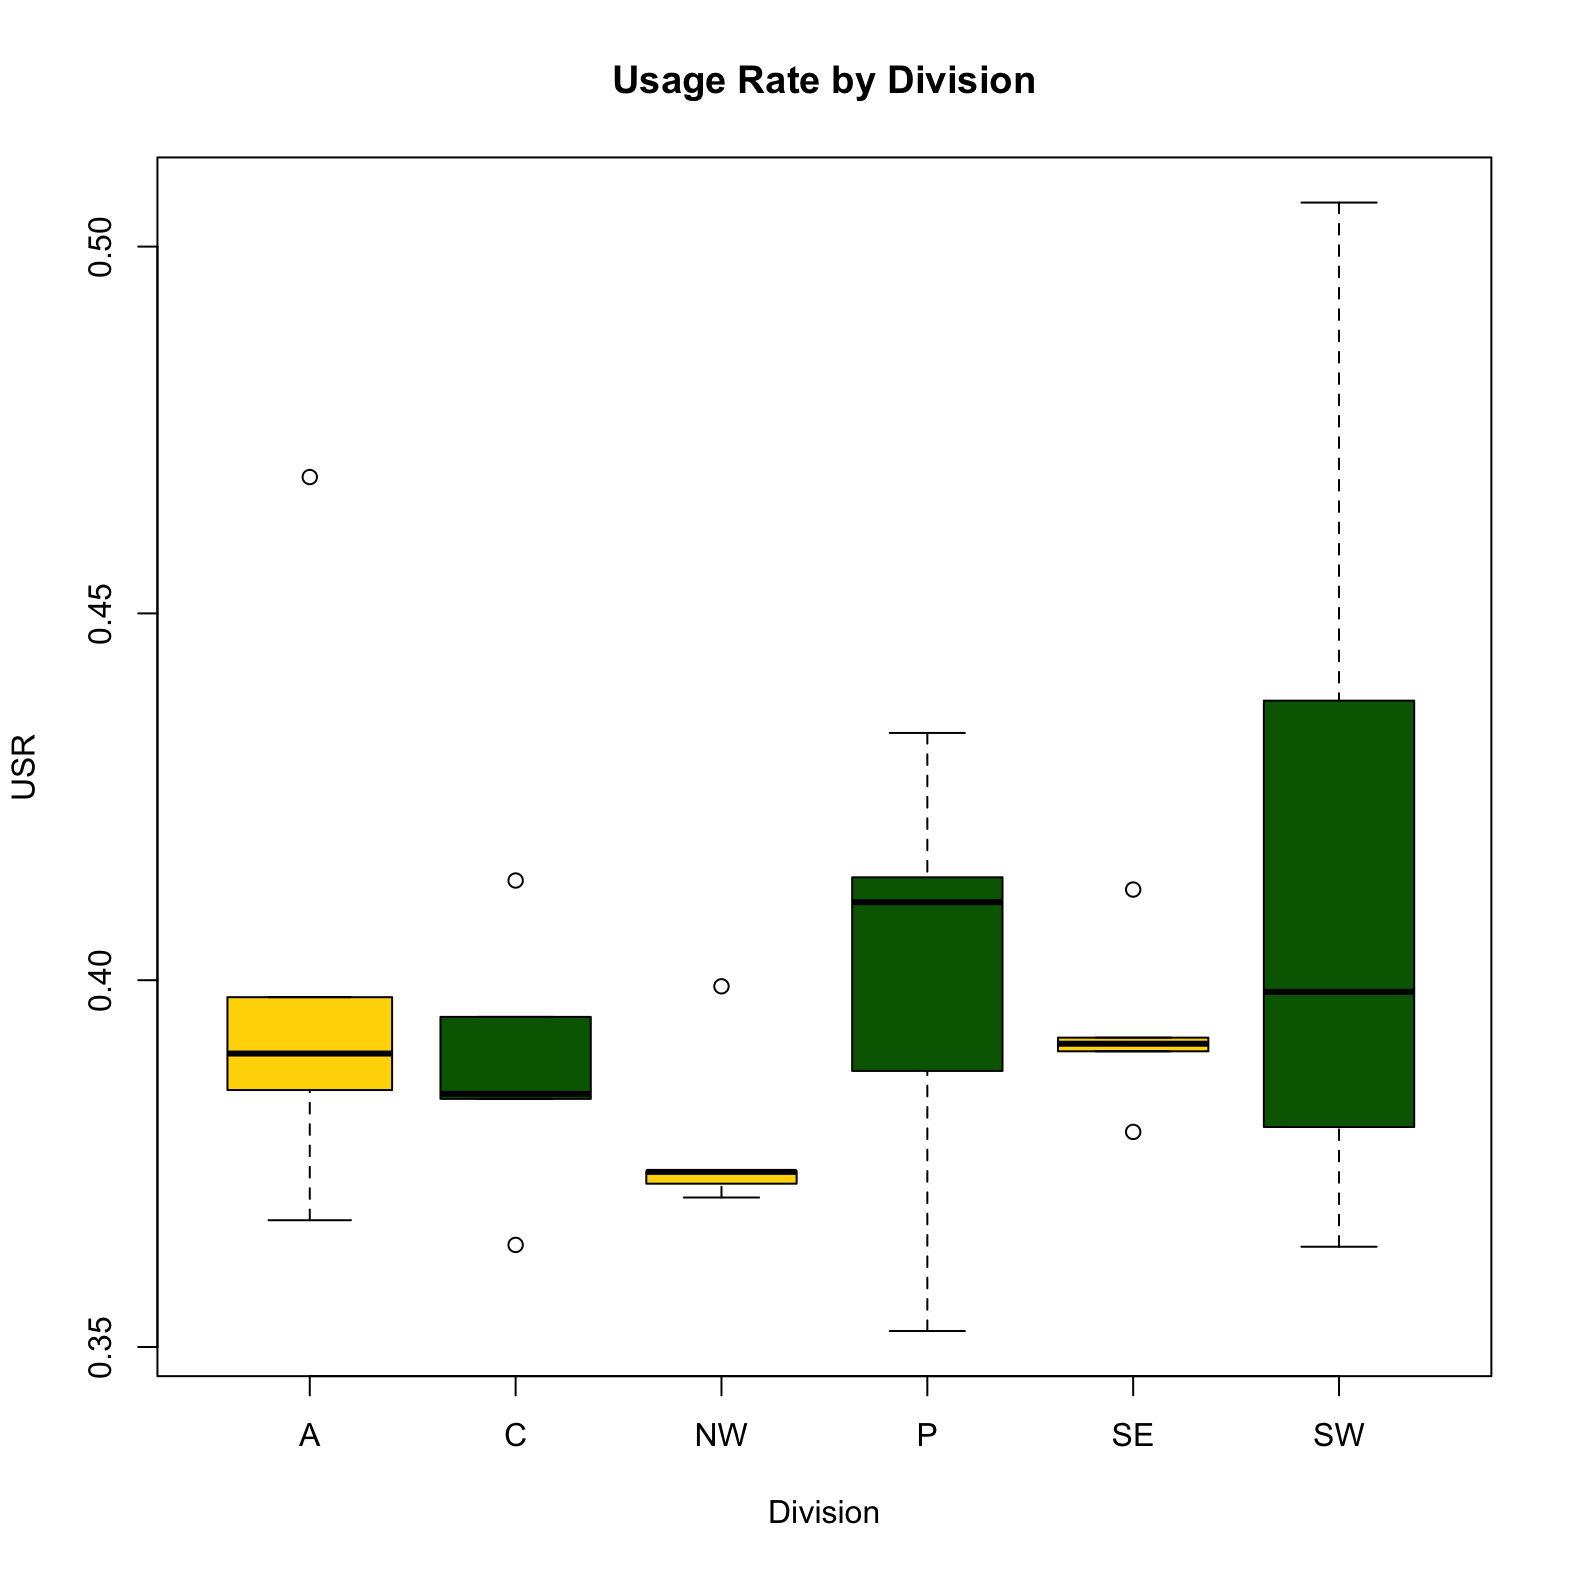
\includegraphics[width=0.9\linewidth, height=5cm]{USRbp.png} 
		\caption{球员利用率箱线图}
		\label{fig:14}
	\end{subfigure}
	\begin{subfigure}{0.5\textwidth}
		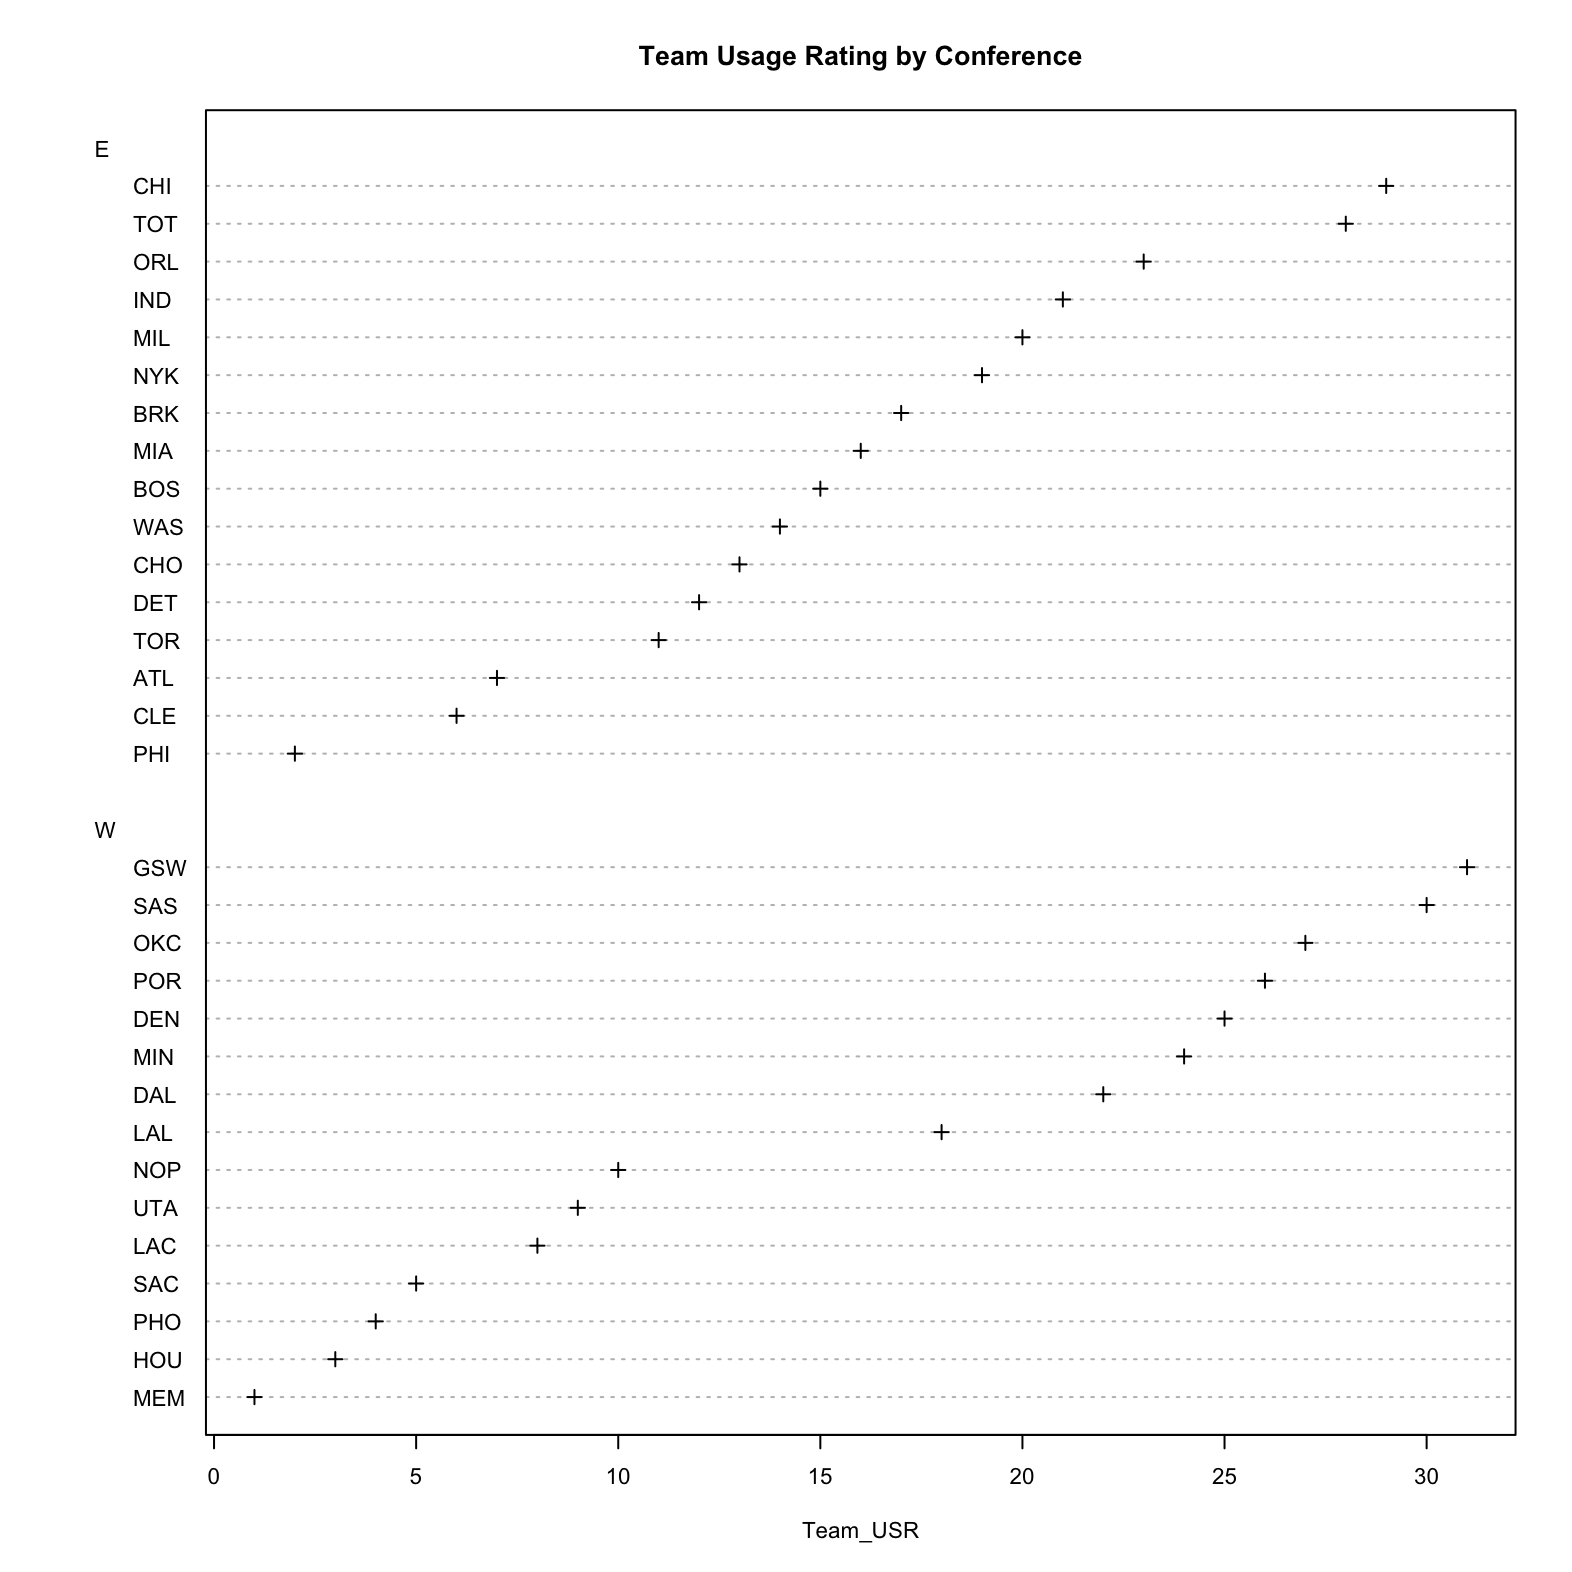
\includegraphics[width=0.9\linewidth, height=5cm]{USRdotp.png}
		\caption{球员利用率散点图}
		\label{fig:15}
	\end{subfigure}
	\caption{球员利用率统计描述}
\end{figure}

	\end{enumerate}






计算指标的均值,中位数,标准差,最大最小值如下表\ref{tab:3}
	\begin{table}[h!]
	\centering
	\begin{tabular}{|c|c|c|c|c|c|}
		\hline
		变量名	          &       Mean &     Median &        Sd         &Max     &    Min\\
		\hline
		W/L\%   &     0.5066452  & 0.5120000 &0.14895694  & 0.7320000 &  0.2070000\\
		MOV/A   &    0.1777419 & -0.4000000 &4.73044164   &8.0500000 & -9.3900000\\
		ORtg/A&    111.1574194 &111.2900000 &2.97113779 &116.6000000 &105.3100000\\
		DRtg/A   & 110.9838710 &110.9700000 &2.91391224 &118.6400000 &105.9400000\\
		NRtg/A     & 0.1719355 & -0.3600000 &4.72743159 &  7.6600000 & -9.8200000\\
		Team\_TSR   & 0.3960872 &  0.3862271 &0.04288839  & 0.5036835  & 0.3181109\\
		Team\_eFGP  & 0.4028148  & 0.4006380 &0.06063737  & 0.5459727   &0.3060132\\
		Team\_USR   & 0.3960933 &  0.3903063 &0.03155086   &0.5060015 &  0.3521769\\
		Team\_PER  &  0.3952573 &  0.3985277& 0.03407403 &  0.4677711 &  0.3392575\\
		Team\_Poss &102.3579355& 102.3520000& 0.34456368 &102.8720000 &101.6280000\\
		\hline
	\end{tabular}
	\caption{描述统计分析}
	\label{tab:3}
\end{table}

胜率的最小值是0.2,最大值是0.7说明最优秀的球队在比赛中有70\%的可能性获胜,最差的球队在比赛中有20\%的获胜率,标准差是0.14,中位数和均值是0.5;说明一般球队的胜率是50\%,也就是这些球队的水平是中间位置,比他强和弱的球队各占50\%。
 比分差距变量最大值是8分,最小值是-9分,即一个球队平均最高可以以8分的差距胜出,最小可以以9分的差距失败,平均水平是0分。标准差是4.73分,即球队之间比分差距变量的分布差距较大。
攻击效率的最高值可达每100次进攻116分,最低不低于每100次进攻105分,平均水平在每100次进攻可获得110分,标准差是3分,即每个球队进攻得分相差不大。
	 防守效率最高可达118分,最低不低于105分,代表对方球队每进攻100次,可以得到118分,最低可得到105分。中位数是110分。标准差是3分,即每个球队的防守失分相差不大。
	 净得分与比分差距的含义相似,分布也相似,在这里可以怀疑这两个变量具有很高的相关性。
	球队球员的实际命中率的平均值是0.39,说明一个球队的球员每投一次球平均有30\%的可能性投进,最高值可达50\%,说明这个优秀的球队每个球员平均都有50\%可能性投篮命中,最低不低于0.3,说明这个球队球员平均只有30\%的可能性投进。标准差是0.04,说明球员实际命中率指标的差距不大。
	球员有效得分率的中位数是0.4,最大值是0.54,说明一个优秀的球队每个球员得分效率可达54\%,最小值是0.31,一个较差的球队得分效率不低于31\%,标准差是0.06,说明球员得分效率变量个体之间差距不大。
	 球队球员利用率平均值是0.39,最大值是0.55,说明这个球队球员在控球时球队对其利用率是55\%,最小值是0.30,一个较差的球队球员在控球时球队对其的利用率不低于30\%,标准差是0.03说明球队之间球员利用效率差距不大,分布较为集中。
	 球队球员效率的平均值是0.39,最大值是0.46,说明球队球员的效率最高平均可达0.46,最小值是0.33说明球队球员的效率最低不低于0.33。
	%插入表格

	

	
	\section{相关性分析}
	在分析后每个指标的统计分布情况后,发现有些变量的极差相差无几,甚至分布情况也大致相同,这里怀疑变量之间存在相关性,并进行相关性分析如下:

\begin{figure}[h!]
	\centering
	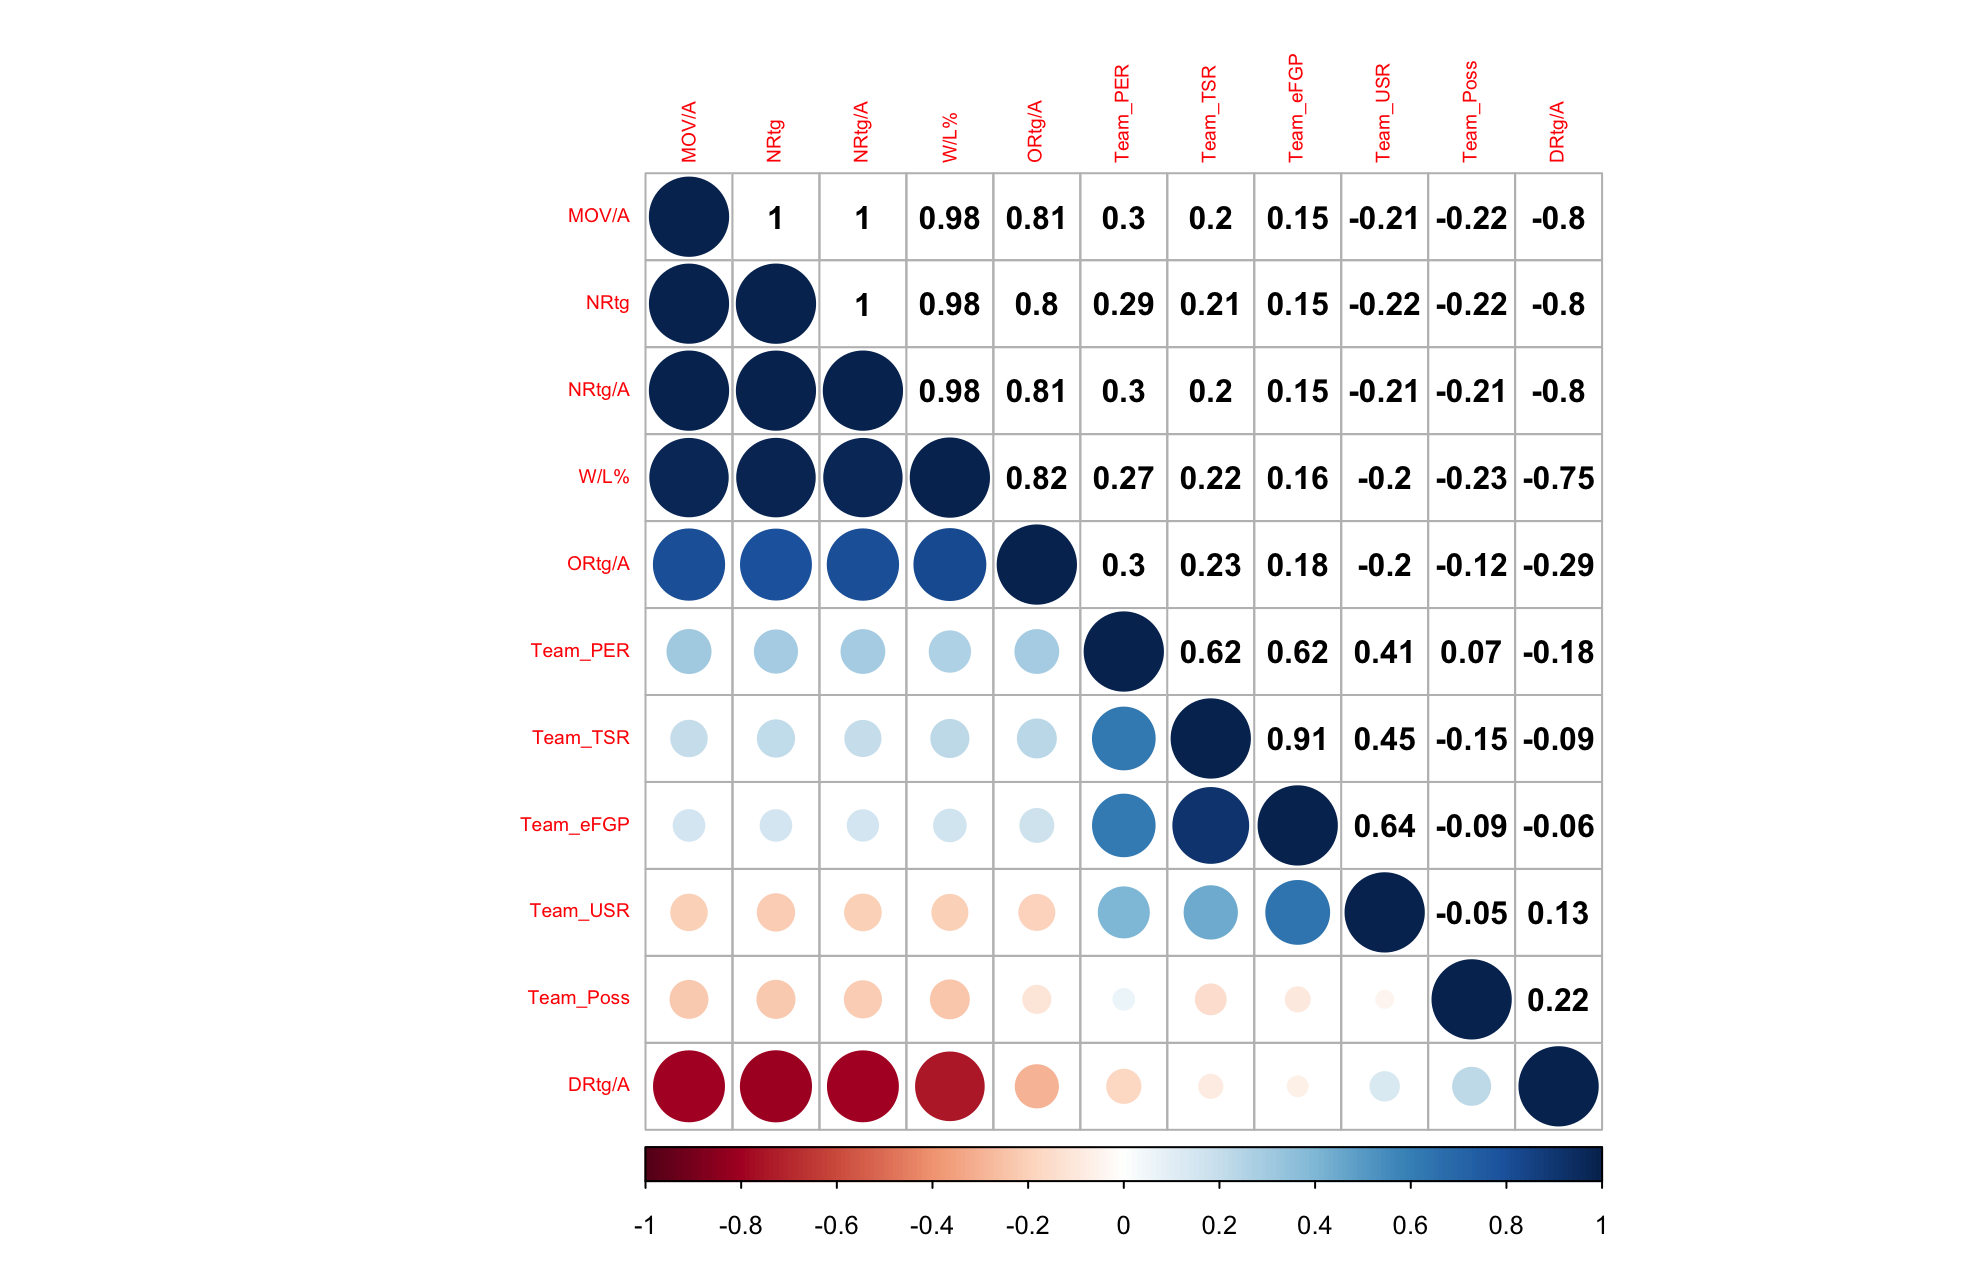
\includegraphics[width=15cm]{corr.png}\label{fig:16}
	\centering
	\caption{变量相关图}
\end{figure}

上图中蓝色代表变量之间有正相关,红色代表变量之间有负相关关系,蓝色越深面积越大说明变量之间的正相关关系越强,对角线是变量自身的相关性,是完全相关相关系数为1,但是净得分和比分差距与胜率之间有1的相关性,这里可以认为净得分和比分差距是完全共线性,可以认为这两个变量是相同的,剔除比分差距这个变量。胜率和净得分有0.98的高度相关性,说明球队净得分越高,则球队的胜率越高,由于两者相关性过高,在建模时容易覆盖其他变量对因变量的影响,所以去除净得分变量。球队进攻效率和胜率之间的相关性是0.81,说明进攻效率越高,球队获胜可能性越高,而防守效率与球队胜率之间有-0.8的相关性,即防守失分率越低,球队获胜可能性越高,防守失分率和进攻效率之间有-0.29的相关性,说明防守效率和进攻效率并不是很强的相关;球员效率与胜率有0.3的正相关性,说明球员效率越高,球队获胜的可能性越大;球员的利用率与胜率之间有0.27 的相关性,说明球员的利用率越高,球队获胜的可能性越大;球员利用率和球员的有效得分率之间有0.64的正相关,说明一个球员在控球时打出越高的有效得分说明球员的利用率越高。
\\

根据上述结论,我们剔除与胜率有极大相关性的变量,研究球队胜率W/L\%(因变量),球队攻击效率ORtg/A, 球队防守效率DRtg/A, 球队实际命中率Team\_TSR,,球队球员有效得分率Team\_eFGP,球队有效利用率Team\_USR,球队整体球员效率Team\_PER,球队控球次数Team\_Poss这8个变量对球队胜率的影响大小。

	
	\section{模型建立}
	多元线性回归模型:
本文最终采用的建模变量包括:球队胜率W/L\%(因变量),球队攻击效率ORtg/A, 球队防守效率DRtg/A, 球队实际命中率Team\_TSR,,球队球员有效得分率Team\_eFGP,球队有效利用率Team\_USR,球队整体球员效率Team\_PER,球队控球次数Team\_Poss这8个变量对球队胜率的影响大小。将变量标准化之后建立模型结果如下:



\begin{table}[h!]
	\begin{tabular}{|c|c|c|c|c|}
		\hline
		\multicolumn{5}{|c|}{Call:lm(formula = `W/L\%` ~ ., data = data\_scale)} \\
		\hline
		\multicolumn{5}{|c|}{ Residuals:} \\
		\hline
		     Min   &    1Q&   Median&       3Q &     Max \\
		-0.47970& -0.10857 & 0.05285 & 0.14674  &0.29542\\
		\hline
		 \multicolumn{5}{|c|}{Coefficients}\\
		 \hline
		            &  Estimate& Std. Error& t &value Pr(>|t|)\\  
		 (Intercept) &-9.087e-15 & 3.965e-02  & 0.000 &  1.0000  \\
		 `ORtg/A`   &  1.344e+01 & 2.339e+01 &  0.575  & 0.5713  \\
		 `DRtg/A` &   -1.308e+01&  2.292e+01  &-0.571  & 0.5741  \\
		 Team\_TSR   &  1.550e-01 & 1.237e-01  & 1.252 &  0.2236 \\
		 Team\_eFGP &  -1.239e-01 & 1.397e-01 & -0.887 &  0.3848  \\
		 Team\_USR &    5.092e-02 & 7.117e-02&   0.716 &  0.4818  \\
		 Team\_PER  &  -1.032e-01 & 5.833e-02&  -1.769  & 0.0907 .\\
		 Team\_Poss  & -2.781e-03 & 4.540e-02&  -0.061 &  0.9517  \\
		 \hline
	\multicolumn{5}{|c|}{Signif. codes:  0 ‘***’ 0.001 ‘**’ 0.01 ‘*’ 0.05 ‘.’ 0.1 ‘ ’ 1}\\
	\hline
	\multicolumn{5}{|c|}{Residual standard error: 0.2207 on 22 degrees of freedom}\\
	\hline 
	\multicolumn{5}{|c|}{Multiple R-squared:  0.9643,	Adjusted R-squared:  0.9513 }\\
	\hline
	\multicolumn{5}{|c|}{F-statistic: 74.21 on 8 and 22 DF,  p-value: 3.997e-14}\\
	\hline
	\end{tabular}
	\centering
	\label{tab:9}
	\caption{线性回归模型结果}
\end{table}

结果如上表,根据F检验,得到P值小于0.0001,得到整体模型是高度显著的,说明模型中至少一个自变量对因变量有显著影响。且判决系数R\^2是0.95,说明模型中自变量可以在很大程度解释因变量。说明我们选取的自变量涵盖大量因变量的信息。但由于每一个自变量做自身t检验的显著性都相当低,考虑变量之间是否存在多重共线性。\\

首先做多重共线性检验,结果如下:
\begin{table}[h!]
	\begin{tabular}{|c|c|c|}
		\hline
		   `ORtg/A`   &  Team\_Pos &    Team\_TSR   \\ 	
		3.367558e+05 &1.269040e+00   &9.425593e+00\\
		\hline
			   Team\_eFGP  &   Team\_USR  &   Team\_PER  \\
		 1.202196e+01 &3.117979e+00 &2.094777e+00  \\
		\hline
	\end{tabular}
\centering
\caption{方差膨胀因子}
\label{tab:8}
\end{table}

可以看出进攻效率的方差膨胀因子达到10\^5,其他变量的方差膨胀因子不超过10,说明变量之间存在多重共线性。我们采取三种方法消除多重共线性,返回模型,并进行比较。

\begin{enumerate}
	\item {\bfseries 直接去除方差膨胀因子大的变量建模结果如下}
	\begin{table}[h!]
		\begin{tabular}{|c|c|c|c|c|}
			\hline
			\multicolumn{5}{|c|}{ Residuals:} \\
			\hline
			Min  &    1Q&  Median  &    3Q    & Max \\
			-1.5776& -0.6801  &0.0569  &0.5126 & 1.6552 \\
			\hline
			\multicolumn{5}{|c|}{Coefficients}\\
			\hline
			&  Estimate& Std. Error& t &value Pr(>|t|)\\  
			(Intercept) &-5.624e-15  &1.534e-01 &  0.000  & 1.0000  \\
			Team\_TSR  &  -4.243e-01 & 4.567e-01 & -0.929&   0.3617  \\
			Team\_eFGP  &  7.025e-01 & 5.111e-01 &  1.374   &0.1815  \\
			Team\_USR   & -6.275e-01 & 2.326e-01&  -2.698&   0.0123 *\\
			Team\_PER  &   4.799e-01 & 1.866e-01  & 2.572   &0.0164 *\\
			Team\_Poss  & -3.058e-01&  1.622e-01 & -1.885  & 0.0711 .\\
			\hline
			\multicolumn{5}{|c|}{Signif. codes:  0 ‘***’ 0.001 ‘**’ 0.01 ‘*’ 0.05 ‘.’ 0.1 ‘ ’ 1}\\
			\hline
			\multicolumn{5}{|c|}{Residual standard error: 0.2207 on 22 degrees of freedom}\\
			\hline 
			\multicolumn{5}{|c|}{Multiple R-squared:  0.3922,	Adjusted R-squared:  0.2707 }\\
			\hline
			\multicolumn{5}{|c|}{F-statistic: 3.227 on 5 and 25 DF,  p-value: 0.02202}\\
			\hline
		\end{tabular}
		\centering
		\label{tab:10}
		\caption{去掉方差膨胀因子过大的变量后线性回归模型结果}
	\end{table}
	
		\begin{figure}[h!]
		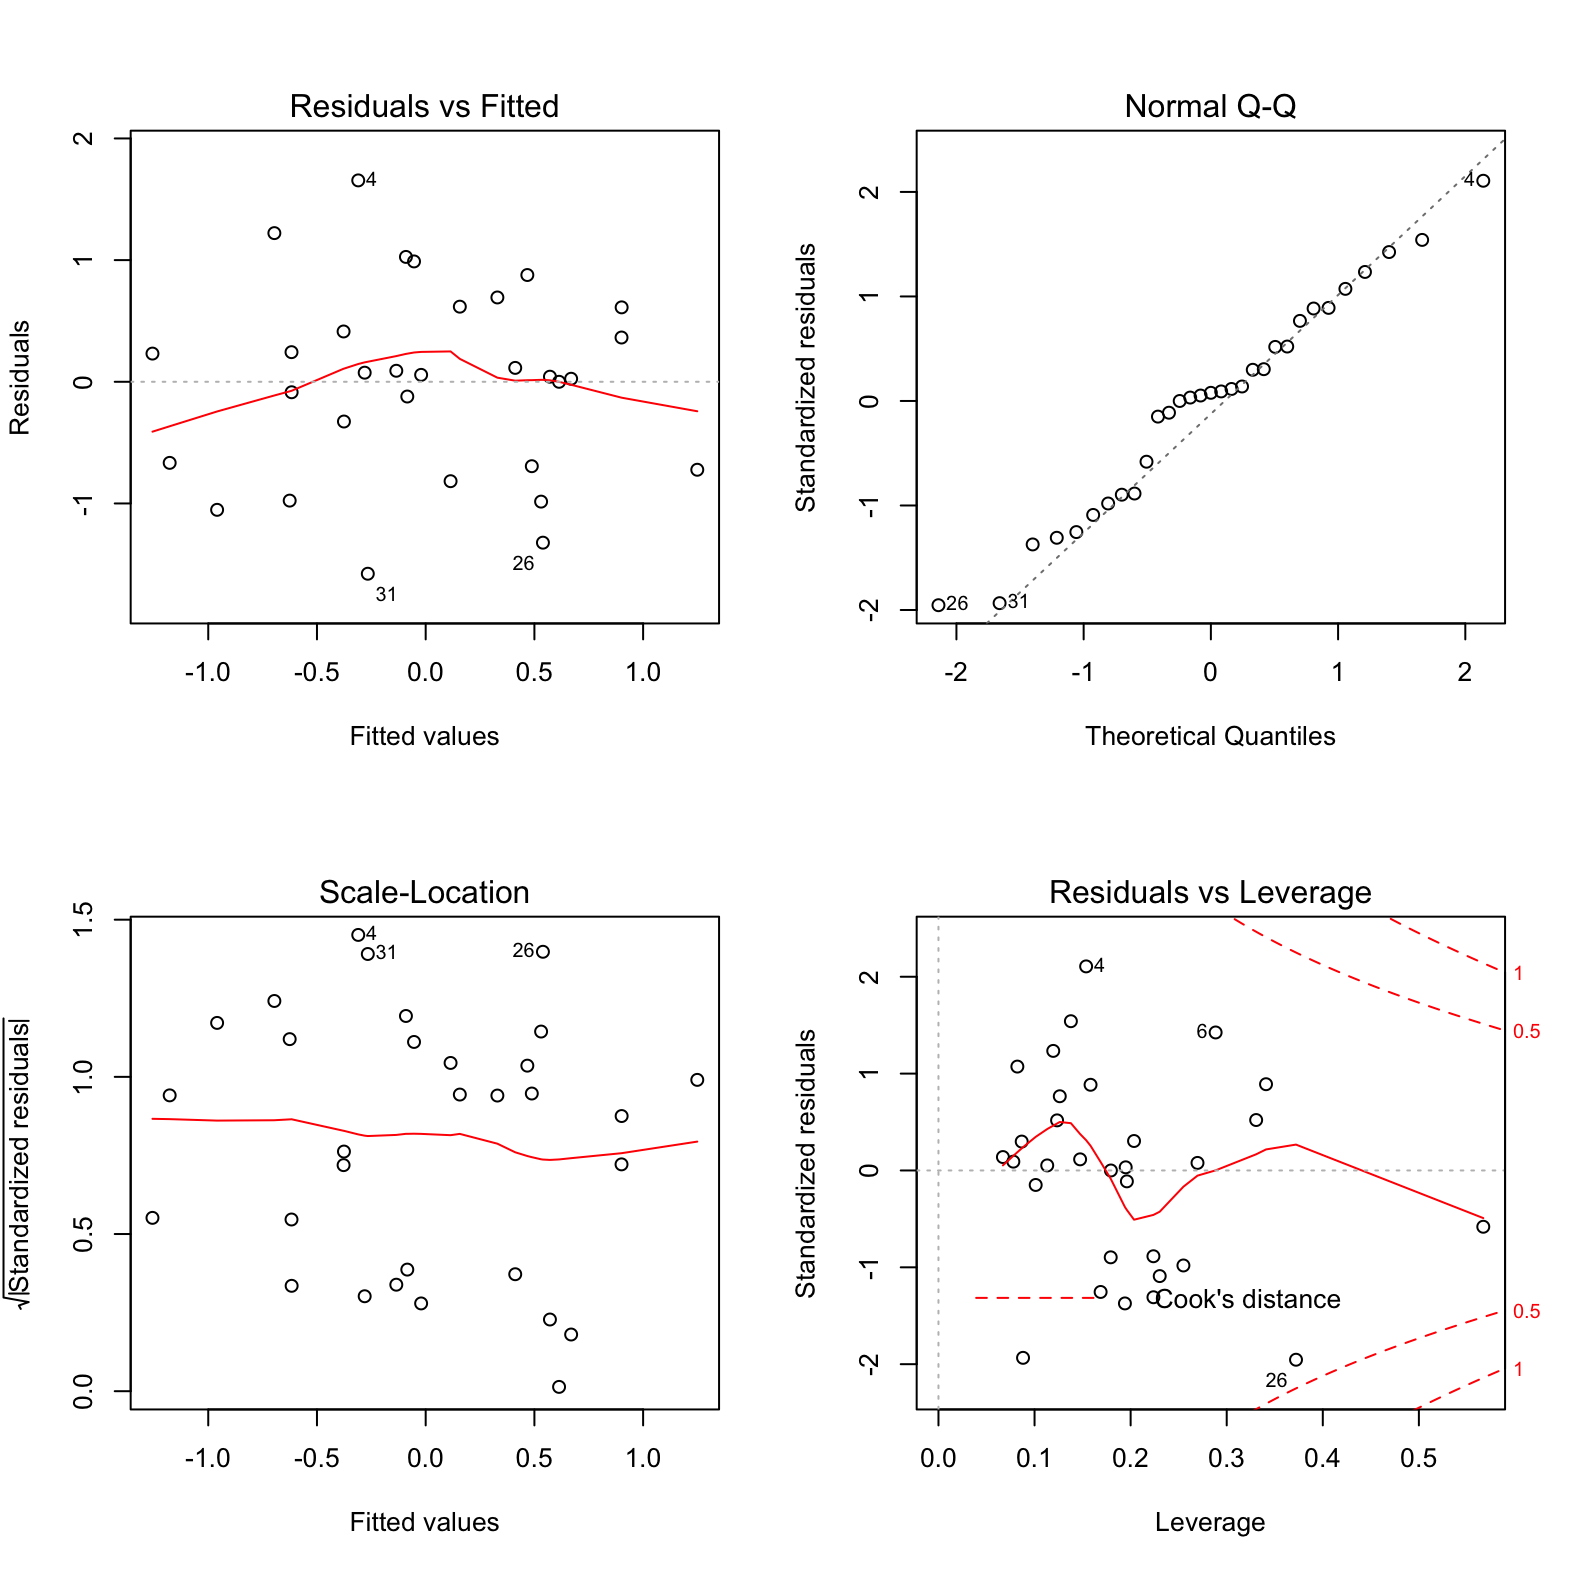
\includegraphics[width=8cm]{regP.png}
		\centering
		\caption{残差分析图}
		\label{fig:17}
	\end{figure}
	由上图可知,残差是正态分布,落在[-2,2]之间,存在极端值第4、31、26个观测对模型有一定影响。
	
	从上图中可以看出,该模型通过F检验后显著性为0.022,在显著性水平为95\%的条件下,模型是显著的,即上述变量中存在可以对球队胜率有影响的变量,模型的R\^2是0.27,说明所选的自变量对球队胜率只可以解释27\%,在本文选择的指标之外,还有73\%的未知因素对球队胜率有影响。每个便利那个的t检验,在95\%显著性下,只有球员利用率和球员效率和球队控球时间对球队胜利概率有显著影响。球员利用率越高,球队胜率越低,球员效率越高,球队胜率越高,球队球员控球时间越长,球队的胜率越低。\\
	
	


	
\item {\bfseries 主成分分析建模:}由于本模型的变量个数较多,且存在一定的相关性,如果分别对每个指标进行分析,往往是孤立的,不能完全利用数据中的信息,且盲目减少指标会损失很多有用的信息,产生错误的结论。在此利用主成分分析,将n维变量映射到k维数据上。PCA的主要思想是将n维特征映射到k维上,这k维是全新的正交特征也被称为主成分,是在原有n维特征的基础上重新构造出来的k维特征。PCA的工作就是从原始的空间中顺序地找一组相互正交的坐标轴,新的坐标轴的选择与数据本身是密切相关的。其中,第一个新坐标轴选择是原始数据中方差最大的方向,第二个新坐标轴选取是与第一个坐标轴正交的平面中使得方差最大的,第三个轴是与第1,2个轴正交的平面中方差最大的。
\\
将上述6个变量进行主成分分析,得到主成分因子的累积贡献率如下:
\begin{table}[h]
	\begin{tabular}{|c|c|c|c|c|c|c|}
		\hline
		\multicolumn{7}{|c|}{ Importance of components:} \\
		\hline
		                        & Comp.1&     Comp.2  &     Comp.3     &  Comp.4    &   Comp.5   &    Comp.6\\
		Standard deviation  &   2.923 &0.337 &0.0742 &2.424e-02&2.227e-02 &1.032835e-02\\
		Proportion of Variance& 0.986&0.013& 0.001& 6.71e-05& 5.726e-05 &1.231e-05\\
		Cumulative Proportion & 0.986& 0.999& 0.99986 &1.00e+00& 1.00e+00 &1.00e+00\\
		\hline
	\end{tabular}
\end{table}
可以看到从第四个主成分开始就已将涵盖了这六个变量的全部信息,我们查看前三个变量的因子载荷矩阵:

 得到第一个主成分$Pc1 =  ORtg\_A    $ ,第二个主成分为$Pc2 = Team\_Poss$, 第三个主成分为$Pc3 = 0.515*Team\_TSR+0.780*Team\_eFGP+0.298 *Team\_USR+0.194*Team\_PER$,说明球队自身的数据涵盖了更多关于球队是否可以获胜的信息,而根据球员数据得到的数据,整体构成了第三个主成分。
 
                      
\begin{table}[h]
	\begin{tabular}{|c|c|c|c|}
		\hline
		\multicolumn{4}{|c|}{Loadings:}\\
		\hline
		Variable	&Comp.1 &Comp.2& Comp.3 \\
		ORtg\_A   &  1.000    & 0& 0\\                              
		Team\_TSR   &   0       & 0&  -0.515\\ 
		Team\_eFGP  & 0&    0&         -0.780 \\
		Team\_USR     &0&0       &    -0.298 \\ 
		Team\_PER  &0&       0&       -0.194\\  
		Team\_Poss     &0&   1.000  &0\\    
		\hline                      
	\end{tabular}
	\centering
	\label{tab:11}
	\caption{主成分因子载荷}
\end{table}

这里做主成分回归,选择三个主成分,采用的最优量化指标为均方根误差RMSEP,得到最终的模型为:

\begin{multline}
  W/L\% = 0.572*ORtg/A+0.110*Team\_TSR+0.0134*Team\_eFGP-0.286*Team\_USR+\\0.228*Team\_PER-0.193*Team\_Poss
\end{multline}




\item {\bfseries 岭回归建模}
最小二乘法的局限性是当变量之间的相关性较强(多重共线性),自变量矩阵不再是满秩矩阵。那就会使得($X^{T}X$)的结果趋近于0,造成拟合参数的数值不稳定性增加(参数间的差距变化很大)。岭回归可以被看作为一种改良后的最小二乘法,它通过向损失中添加L\_{2}正则项(2-范数)有效防止模型出现过拟合,且有助于解决非满秩条件下求逆困难的问题,从而提升模型的解释能力。岭回归的损失函数变为:$L_{loss}=||Y-X'W||^2+\lambda ||W||^2$,得到的参数W的表达式为$W=(X^TX+\lambda I)^{-1}X^TY$
利用岭回归建模得到如下结果:
\begin{table}[h]
	\begin{tabular}{|c|c|c|c|c|c|}
		\hline
		\multicolumn{6}{|c|}{Coefficients:}\\
		\hline
		& Estimate &Scaled estimate& Std. Error (scaled)& t value (scaled) &Pr(>|t|)   \\
		  (Intercept)& -3.287e-15  &            NA   &               NA      &         NA  &     NA  \\
		    `ORtg/A`   &  6.501e-01  &     3.561e+00       &    5.995e-01      &      5.939 &2.87e-09 ***\\
		    Team\_TSR &   -2.988e-02&      -1.636e-01  &         7.226e-01    &        0.226  &  0.821    \\
		    Team\_eFGP &   7.847e-02  &     4.298e-01  &         7.448e-01     &       0.577   & 0.564   \\ 
		    Team\_USR &   -1.477e-01 &     -8.091e-01     &      6.482e-01   &         1.248  &  0.212  \\  
		    Team\_PER   &  1.489e-01&       8.153e-01       &    6.313e-01     &       1.291   & 0.197   \\ 
		    Team\_Poss   &-1.600e-01 &     -8.765e-01   &        5.504e-01   &         1.593 &   0.111   \\ 
		    \hline
		    \multicolumn{6}{|c|}{Signif. codes:  0 ‘***’ 0.001 ‘**’ 0.01 ‘*’ 0.05 ‘.’ 0.1 ‘ ’ 1}\\
		    \hline
		     \multicolumn{6}{|c|}{Ridge parameter: 0.09169586, computed using 4 PCs}\\
		     \hline
		     \multicolumn{6}{|c|}{Degrees of freedom: model 4.812 , variance 4.13 , residual 5.493}\\
		     \hline
	\end{tabular}
\centering
\end{table}
该模型得到结果如上表所示,可以看出只有ORtg/A即进攻效率是显著影响球队胜率的,该模型自动选取岭回归参数0.0917,选取了4个主成分,得到的最终模型为:
\begin{multline}
W/L\% =-3.287e-15+ 0.6501*ORtg/A-0.02988*Team\_TSR+0.07847*Team\_eFGP-\\0.1477*Team\_USR+0.1489*Team\_PER-0.16*Team\_Poss
\end{multline}


\end{enumerate}






  



	
	\section{模型评估与结论}
	{\bfseries 根据上述三个纠正后的模型得到如下模型结果:}
\begin{figure}[h!]
	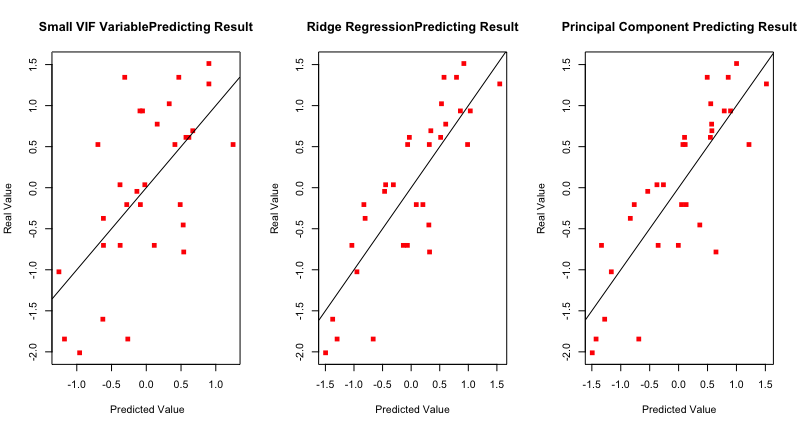
\includegraphics[width=10cm]{Conclusion.png}
	\centering
	\caption{预测结果}
	\label{fig:18}
\end{figure}
看出通过第一种纠正方式,即简单除去膨胀因子过大的变量,导致预测值和真实值在$y=x$两侧的离散程度较大,三个图中,岭回归模型预测的结果是最优的。
比较三组纠正模型的MSE值可得到:
\begin{table}[h]
	\begin{tabular}{|c|c|c|}
		\hline
		Small VIF Variable& Ridge Regression &Principal Component Regression\\
		0.738011&0.5321579&0.5543356\\
		\hline
	\end{tabular}
\centering
\end{table}
由上表结论可知,岭回归模型在这里的表现最好,本文采用岭回归模型进行预测NBA球员数据和球队胜率的关系会得到更好的结果。\\



{\bfseries 模型评价:}由于本文试图通过公开的数据和建模寻找球员表现和球队胜负的关系,其中一些不可控因素会导致模型出现一定的问题,例如,一些球员在赛季中受伤退赛或者没有退赛但是伤势会对其表现有很大的影响;或者某些球员在某一赛季中因选秀被交易到其他球队效力;或者某队在赛季中因更换教练导致球队风格有了很大的改变;或者某些球队的数据过于相似而导致其特征不够显著而无法得到更精准的预测。\cite{yang2015predicting}
\\
此外我们得到我们的变量对因变量具有一定的解释作用,其中球员实际命中率每增加1\%,球队的胜率会降低0.42\%,
球员有效得分率每提高1\%,球队获胜的概率会上升0.71\%,球员使用率每上升1\%,就会对球队造成胜率下降0.63\%的影响,而球员效率每提高1\%就会对球队获胜的概率提升0.48\%,球队控球时间越长就会对球队的胜率影响不利;该模型说明,当球队在制定训练方案时应着重注意的是提升球员的个人效率,降低球队对每位球员的使用效率,不仅要提高球员的投篮命中率,还有增强球员之间的团结合作,提升有效得分率。最终要严格控制每场比赛球队在场上的控球时间,这样可以节省运动员体能,获得更精彩的发挥。
	
	

	\bibliography{Ref}
	
	
	\section{代码部分}
	\begin{lstlisting}[language=R,caption=My code]
	library(dplyr)
	library(readxl)
	library(ggplot2)
	library(e1071)
	library(gridExtra)
	library(DMwR)
	library(rpart)
	library('MASS')
	library(ridge)
	library(corrplot)
	library(car)
	Player_sta <- read_xlsx("/Users/sun/Desktop/NBA/2018-19.xlsx",sheet="Player_sta",col_names=T,na="NA")
	Team_Name <- read_xlsx("/Users/sun/Desktop/NBA/2018-19.xlsx",sheet="Team_Name",col_names=T,na="NA")
	Team_Result <- read_xlsx("/Users/sun/Desktop/NBA/2018-19.xlsx",sheet="Team_Result",col_names=T,na="NA")
	Team_sta <- read_xlsx("/Users/sun/Desktop/NBA/2018-19.xlsx",sheet="Team_sta",col_names=T,na="NA")
	Opponent_sta <- read_xlsx("/Users/sun/Desktop/NBA/2018-19.xlsx",sheet="Opponent_sta",col_names=T,na="NA")
	
	
	
	Team_Result <- right_join(Team_Name,Team_Result,by=c("Full Name"="Full Name"))
	Team_sta <- right_join(Team_Name,Team_sta,by=c("Full Name"="Full Name"))
	Opponent_sta <- right_join(Team_Name,Opponent_sta,by=c("Full Name"="Full Name"))
	Player_sta <- full_join(Team_sta,Player_sta,by=c("Short Name"="Tm"),keep=F)
	Player_sta <- full_join(Team_Result,Player_sta,by=c("Short Name"="Short Name"),keep=F)
	Player_sta <- full_join(Opponent_sta,Player_sta,by=c("Short Name"="Short Name"),keep=F)
	#x是team sta,y是player sta,没有东西是oppo sta
	
	#数据描述
	plot(Player_sta$PTS,Player_sta$PTS.x,main="Offensive and Defensive Ratings in 2018-19",
	xlab="Offensive ratings",ylab="Defensive ratings",col="red",pch=3)
	abline(v=112,h=110,col = "gray60",lty=2)
	
	
	
	
	
	
	
	VOP = Player_sta$PTS / (Player_sta$FGA - Player_sta$ORB + Player_sta$TOV + 0.44 * Player_sta$FTA)
	DRB_percentage = (Player_sta$TRB - Player_sta$ORB) / Player_sta$TRB
	factor = (2/3)-(0.5*(Player_sta$AST/Player_sta$FG))/(2*(Player_sta$FG/Player_sta$FT))
	#构建PER
	uPER = (1/Player_sta$MP.y)*(Player_sta$`3P.y`+(2/3)*Player_sta$AST.y+
	(2-factor*(Player_sta$AST.x/Player_sta$FG.x))*Player_sta$FG.y+
	(0.5*Player_sta$FT.y*(1+(1-(Player_sta$AST.x/Player_sta$FG.x))+(2/3)*
	(Player_sta$AST.x/Player_sta$FG.x)))-VOP*Player_sta$TOV.y-VOP*DRB_percentage*
	(Player_sta$FGA.y-Player_sta$FG.y)-VOP*0.44*(0.44+(0.56*DRB_percentage))*
	(Player_sta$FTA.y-Player_sta$FT.y)+VOP*(1-DRB_percentage)*(Player_sta$TRB.y-
	Player_sta$ORB.y)+VOP*DRB_percentage*Player_sta$ORB.y+VOP*Player_sta$STL.y+
	VOP*(1-DRB_percentage)*(Player_sta$TRB.y-Player_sta$ORB.y)+VOP*DRB_percentage*
	Player_sta$ORB.y+VOP*Player_sta$STL.y+VOP*DRB_percentage*Player_sta$BLK.y-
	(Player_sta$FT-Player_sta$PF)-0.44*VOP*(Player_sta$FTA/Player_sta$PF))
	#构建possesion
	Possesion_team <- Player_sta$FGA.x+0.44*Player_sta$FTA.x-Player_sta$ORB.x+Player_sta$TOV.x
	Possesion_opp <-  Player_sta$FGA+0.44*Player_sta$FTA-Player_sta$ORB+Player_sta$TOV
	#构建节奏调整
	Pace_adjust <- Possesion_opp/Possesion_team
	PER_adjust <- uPER*Pace_adjust
	
	#构建Usage percentage rate
	USR <- ((Player_sta$FGA.y  + 0.44 *Player_sta$FTA.y +Player_sta$TOV.y) * (Player_sta$MP.x / 5)) / 
	( Player_sta$MP.y * (Player_sta$FGA.x + 0.44 * Player_sta$FGA.x + Player_sta$TOV.y))
	
	#构建Effective Field Goal Percentage
	eFGP <- (Player_sta$FG.y  + 0.5 * Player_sta$`3P.y`) / Player_sta$FGA
	
	#构建TRUE shooting Rate
	TSA <-  Player_sta$FGA.y + 0.44 * Player_sta$FTA.y
	TSR <- Player_sta$PTS.y  / (2 * TSA)
	
	#构建总体关于“率”的团队计算法###########
	RATING <- function(x,y){
	return(x*y/sum(x*y,na.rm = T))
	}
	
	TSR_min <- RATING(Player_sta$MP.y,TSR)*100
	eFGP_min <- RATING(Player_sta$MP.y,eFGP)*100
	USR_min <- RATING(USR,Player_sta$MP.y)*100
	PER_min <- RATING(PER_adjust,Player_sta$MP.y)*100
	
	Team_TSR <- aggregate(TSR_min,by=list(Player_sta$`Short Name`),mean,na.rm=T)$'x'
	Team_eFGP <- aggregate(eFGP_min,by=list(Player_sta$`Short Name`),mean,na.rm=T)$'x'
	Team_USR <- aggregate(USR_min,by=list(Player_sta$`Short Name`),mean,na.rm=T)$'x'
	Team_PER <- aggregate(PER_min,by=list(Player_sta$`Short Name`),mean,na.rm=T)$'x'
	Team_Poss <- aggregate(Possesion_team,by=list(Player_sta$`Short Name`),mean,na.rm=T)
	
	####组成建模的数据
	Rating_Team <- cbind(Team_TSR,Team_eFGP,Team_USR,Team_PER,Team_Poss)
	colnames(Rating_Team) <- c("Team_TSR","Team_eFGP","Team_USR","Team_PER","Team","Team_Poss")
	data <- right_join(Team_Result,Rating_Team,by=c("Short Name"="Team"))
	data$Conf <- as.factor(data$Conf)
	data$Div <- as.factor(data$Div)
	data <- data[,c(2:8,12:21)]
	summary(data)
	
	####描述性分析
	Mean <- apply(data[7:17], 2, mean,na.rm=T)
	Median <- apply(data[7:17], 2, median,na.rm=T)
	Sd <- apply(data[7:17], 2, sd,na.rm=T)
	Max <- apply(data[7:17], 2, max,na.rm=T)
	Min <- apply(data[7:17], 2, min,na.rm=T)
	as.data.frame(cbind(Mean,Median,Sd,Max,Min))
	
	#######考虑变量间的相关关系画图
	corr <- cor(data[7:17])
	corrplot(corr = corr,order="FPC",type="lower",tl.pos = "lt",tl.cex = 0.6)
	corrplot(corr = corr,add=TRUE, type="upper", method="number",order="FPC", 
	col="black",diag=FALSE,tl.pos="n", cl.pos="n")
	
	###因变量的分布图
	h <-hist(data$`W/L%`,freq = T,breaks=12,main = "Distribution of Wining Ratio",
	xlab="Wining Rate", ylab="Density")
	rug(jitter(data$`W/L%`))
	lines(density(data$`W/L%`), col="blue", lwd=2)
	xfit<-seq(min(data$`W/L%`), max(data$`W/L%`), length=40) 
	yfit<-dnorm(xfit, mean=mean(data$`W/L%`), sd=sd(data$`W/L%`)) 
	yfit <- yfit*diff(h$mids[1:2])*length(data$`W/L%`) 
	lines(xfit, yfit, col="red", lwd=2)
	box() 
	legend(0.2,5,c("Red:Normal","Blue:WinR"),cex=0.6)
	##正态检验
	p1 <- qqPlot(data$`W/L%`,distribution = "norm",envelope = 0.9,main="Normal Test",ylab="WinR")
	y <- pnorm(xfit, mean=mean(data$`W/L%`), sd=sd(data$`W/L%`))
	shapiro.test(data$`W/L%`)
	
	#boxplot
	boxplot(`MOV/A`~Div, data = data,varwidth=TRUE,
	col=c("gold","darkgreen"),main = "Margin of Vicotry by Division",
	xlab = "Division", ylab = "MOV")
	
	boxplot(`ORtg/A`~Div, data = data,varwidth=TRUE,
	col=c("gold","darkgreen"),main = "Offensive Rate by Division",
	xlab = "Division", ylab = "ORtg")
	
	boxplot(`DRtg/A`~Div, data = data,varwidth=TRUE,
	col=c("gold","darkgreen"),main = "Defensive Rate by Division",
	xlab = "Division", ylab = "DRtg")
	
	boxplot(`Team_TSR`~Div, data = data,varwidth=TRUE,
	col=c("gold","darkgreen"),main = "True Shooting Rate by Division",
	xlab = "Division", ylab = "TSR")
	
	boxplot(`Team_eFGP`~Div, data = data,varwidth=TRUE,
	col=c("gold","darkgreen"),main = "Effeciency Field Goal Percentage",
	xlab = "Division", ylab = "eFGP")
	
	boxplot(`Team_USR`~Div, data = data,varwidth=TRUE,
	col=c("gold","darkgreen"),main = "Usage Rate by Division",
	xlab = "Division", ylab = "USR")
	
	boxplot(`Team_PER`~Div, data = data,varwidth=TRUE,
	col=c("gold","darkgreen"),main = "PER by Division",
	xlab = "Division", ylab = "PER")
	
	#dotplot 
	data <- data[order(data$`MOV/A`,decreasing = T),]
	dotchart(order(data$`MOV/A`,decreasing = T), labels=data$`Short Name`, cex=.7,
	main="Margin of Victory by Conference",pch=3,
	xlab="MoV",groups = data$Conf)
	
	data <- data[order(data$`ORtg/A`,decreasing = T),]
	dotchart(order(data$`ORtg/A`,decreasing = T), labels=data$`Short Name`, cex=.7,
	main="Offensive Rating by Conference",pch=3,
	xlab="ORtg",groups = data$Conf)
	
	data <- data[order(data$`ORtg/A`,decreasing = T),]
	dotchart(order(data$`ORtg/A`,decreasing = T), labels=data$`Short Name`, cex=.7,
	main="Offensive Rating by Conference",pch=3,
	xlab="ORtg",groups = data$Conf)
	
	data <- data[order(data$`DRtg/A`,decreasing = T),]
	dotchart(order(data$`DRtg/A`,decreasing = T), labels=data$`Short Name`, cex=.7,
	main="Defensive Rating by Conference",pch=3,
	xlab="DRtg",groups = data$Conf)
	
	data <- data[order(data$Team_TSR,decreasing = T),]
	dotchart(order(data$`Team_TSR`,decreasing = T), labels=data$`Short Name`, cex=.7,
	main="True Shooting Rating by Conference",pch=3,
	xlab="Team_TSR",groups = data$Conf)
	
	data <- data[order(data$Team_USR,decreasing = T),]
	dotchart(order(data$`Team_USR`,decreasing = T), labels=data$`Short Name`, cex=.7,
	main="Team Usage Rating by Conference",pch=3,
	xlab="Team_USR",groups = data$Conf)
	
	data <- data[order(data$Team_PER,decreasing = T),]
	dotchart(order(data$`Team_PER`,decreasing = T), labels=data$`Short Name`, cex=.7,
	main="Team PER by Conference",pch=3,
	xlab="Team_PER",groups = data$Conf)
	
	data <- data[order(data$`Team_Poss`,decreasing = T),]
	dotchart(order(data$`Team_Poss`,decreasing = T), labels=data$`Short Name`, cex=.7,
	main="Team possesion by Conference",pch=3,
	xlab="Team_Poss",groups = data$Conf)
	
	data_scale <- as.data.frame(scale(data[,c(7,10:17)]))
	#data$Team <- data$`Short Name`
	
	#model3 glm
	lm1 <- lm(`W/L%`~.,data=data_scale[c(1,5:9)])
	summary(lm1)
	vif(lm1)
	lm1 <- lm(`W/L%`~.,data=data_scale[c(1,5:9)])
	summary(lm1)
	par(mfrow=c(2,2))
	plot(lm1)
	lm1 <- linearRidge(`W/L%`~.,data=data_scale[c(1,5:9)])
	summary(lm1)
	
	pre_result <- round(predict(lm1,data_scale[c(1,5:9)]),3)
	pre_result <- pre_result*sd(data$`W/L%`)+mean(data$`W/L%`)
	par(mfrow=c(1,1))
\end{lstlisting}







    
	\section{致谢}
	感谢我的论文导师李婷婷老师在大学四年中的谆谆教诲、在论文撰写期间的悉心指导,她的宝贵建议带给我本文的创作灵感,并在她的帮助下得以顺利完成,在此表达我最诚挚的谢意。大学时光眨眼接近尾声,感谢我的母校,感谢每一位老师对我们的栽培,为我们 付出的心血,感谢给予我帮助的朋友、同学,以及在背后默默支持我的家人,是你们引导我、鼓励我勇敢面对困难,使我的生活充满温暖与感动,再一次由衷的表示感谢!

	
	
	
	
	
	
	
	
	
	
\end{document}

